\documentclass[a4paper,13pt]{report}
\usepackage[utf8]{vietnam}
\usepackage[utf8]{inputenc}
\usepackage{amsmath}
\usepackage{amsfonts}
\usepackage{amssymb}
\usepackage{graphicx}
\usepackage[font=small]{caption}
\usepackage{booktabs}
\usepackage[unicode]{hyperref}
\usepackage[left=3cm,right=2cm,top=2.5cm,bottom=3cm]{geometry}
\usepackage{titlesec} 
\usepackage{scrextend}
\usepackage{enumerate}
\usepackage{tikz}
\usepackage{float}
\usepackage{afterpage}
\usepackage{multirow}
\usepackage{sectsty}
\usepackage{tocloft,calc}
\usepackage{listings}
\usepackage{makecell}
\usepackage[sort&compress]{natbib}
\usetikzlibrary{calc}
\usepackage{algorithm}
\usepackage{perpage}
\MakePerPage{footnote} 
\PassOptionsToPackage{table}{xcolor}

\def\changemargin#1#2{\list{}{\rightmargin#2\leftmargin#1}\item[]}
\let\endchangemargin=\endlist 

\changefontsizes{13pt}
\bibliographystyle{unsrt}

\makeatletter
\def\l@figure{\@dottedtocline{1}{1em}{2.2em}}
\def\l@table{\@dottedtocline{1}{1em}{2.2em}}
\renewcommand*{\ALG@name}{Thuật toán}
\makeatother

\sectionfont{\fontsize{15}{15}\selectfont}
\subsectionfont{\fontsize{13}{15}\selectfont}

\titleformat{\chapter}[display]   
{\normalfont\huge\bfseries}{\chaptertitlename\ \thechapter}{0pt}{\LARGE}
\titlespacing*{\chapter}{0cm}{-\topskip}{0pt}[0pt]

\renewcommand{\baselinestretch}{1.3}
\renewcommand{\cftchappresnum}{Chương }
\AtBeginDocument{\addtolength\cftchapnumwidth{\widthof{\bfseries Chương }}}
\setlength{\parskip}{0.4em}
\setlength{\parindent}{0pt}

\begin{document}

% Cover Vietnamese (with supervisors)
\pagenumbering{gobble}
\begin{center}
	
\begin{tikzpicture}[overlay,remember picture]
	\draw [line width=3pt,rounded corners=0pt]
	($ (current page.north west) + (25mm,-25mm) $)
	rectangle
	($ (current page.south east) + (-15mm,25mm) $);
	\draw [line width=1pt,rounded corners=0pt]
	($ (current page.north west) + (26.5mm,-26.5mm) $)
	rectangle
	($ (current page.south east) + (-16.5mm,26.5mm) $);
	\end{tikzpicture}
	\\[1mm]
	\textbf{ĐẠI HỌC QUỐC GIA HÀ NỘI\\TRƯỜNG ĐẠI HỌC CÔNG NGHỆ}
	\\[1cm]
	
\includegraphics[width=0.2\linewidth]{figures/uet}
	\\[0.3cm]
	\textbf{Lê Quang Duy}
	\\[2cm]
	
	\large{\textbf{PHÁT TRIỂN PHẦN MỀM HỖ TRỢ TÌM HIỂU \\ VÀ KHÁM PHÁ DI SẢN VĂN HÓA DÂN TỘC}}
	\\[2.6cm]
	\normalsize{\textbf{LUẬN VĂN TỐT NGHIỆP ĐẠI HỌC HỆ CHÍNH QUY
		\\[2mm]
	Ngành: Công nghệ thông tin}}
\end{center}
\vspace{16mm}
\hspace*{12mm}\textbf{ Cán bộ hướng dẫn: TS. Ngô Thị Duyên}\\[0.8cm]
\hspace*{12mm}\textbf{ Cán bộ đồng hướng dẫn: PGS. TS. Lê Thanh Hà}
\vfill
\begin{center}
	\textbf{HÀ NỘI - 2022}
	\vspace{10mm}
\end{center}
\newpage\cleardoublepage

\begin{center}
\textbf{\large{Lời cam đoan}	}
\end{center}
\addcontentsline{toc}{chapter}{Lời cam đoan}
Em xin cam đoan rằng sản phẩm dự án cùng báo cáo khóa luận này do em độc
lập phát triển dưới sự hướng dẫn của các thầy cô, không sao chép mã nguồn của bất
kỳ cá nhân, tổ chức hay cộng đồng nào khác. Bài báo cáo chưa từng được nộp như
một báo cáo khóa luận tại trường Đại học Công Nghệ - Đại học Quốc Gia Hà Nội
hoặc bất kỳ trường đại học nào khác.
Trong bài báo cáo nếu có sử dụng tài liệu từ nguồn khác, em xin phép được
trích dẫn cụ thể.
Nếu trái những điều cam đoan trên, em xin chịu hoàn toàn trách nhiệm theo
quy định của trường Đại học Công Nghệ - Đại học Quốc Gia Hà nội

\vspace{1cm}
\begin{flushright}
    Hà Nội, năm 2022\\
    Sinh viên thực hiện\\[0.5cm]
    \textbf{Lê Quang Duy}
\end{flushright}
\newpage\cleardoublepage

\begin{center}
\textbf{\large{Lời cảm ơn}	}
\end{center}
\addcontentsline{toc}{chapter}{Lời cảm ơn}

Đầu tiên, cho em xin được cảm ơn cô Ngô Thị Duyên và thầy Lê Thanh Hà đã trực tiếp hướng dẫn cho em trong dự án này. Cảm ơn thầy và cô đã luôn thẳng thắn góp ý và sát sao hỗ trợ để em có thể hoàn thiện dự án ngày càng đầy đủ và đúng thời hạn.

Tiếp đó, em xin cảm ơn TS. Lư Thị Thanh Lê – giảng viên Khoa Các khoa học liên ngành, Trường Đại học KHXH\&NV, Đại học Quốc gia Hà Nội đã tham gia cố vấn cho dự án về phần kiến thức văn hóa, đồng thời cũng trải nghiệm và góp ý để sản phẩm của dự án được hoàn thiện và chỉn chu hơn.

Cuối cùng, em xin cảm ơn các thầy cô giảng viên của Trường Đại học Công Nghệ – Đại học Quốc gia Hà Nội đã luôn tận tình giảng dạy, cung cấp cho em những kiến thức vô cùng cần thiết để em có nền tảng vững chãi khi tham gia vào môi trường phát triển của ngành Công nghệ Thông tin. Em xin hứa sẽ luôn phấn đấu để cống hiến khả năng của mình cho xã hội và đất nước.

Em xin chân thành cảm ơn!

\vspace{1cm}
\begin{flushright}
    Hà Nội, năm 2022\\
    Sinh viên thực hiện\\[0.5cm]
    \textbf{Lê Quang Duy}
\end{flushright}
\newpage\cleardoublepage

\begin{center}
\textbf{\large{Tóm tắt}	}
\end{center}
\addcontentsline{toc}{chapter}{Tóm tắt}

\textbf{Tóm tắt:} Việt Nam có nguồn tài nguyên du lịch phong phú với sự đa dạng về địa lý, cảnh quan và truyền thống văn hóa của 54 dân tộc. Trong đó, du lịch văn hóa là một phân nhánh quan trọng, vừa góp phần quảng bá hình ảnh đất nước tới bạn bè quốc tế, vừa tạo động lực cho thế hệ trẻ khám phá, bảo tồn và phát triển các giá trị văn hóa dân tộc. Tuy nhiên, trải nghiệm của du khách tại các điểm di sản vẫn còn nhiều hạn chế do thiếu công cụ hỗ trợ tương tác và hướng dẫn trực quan.

Luận văn này đề xuất và phát triển ứng dụng \textbf{TMAP}, được tích hợp trong nền tảng \textbf{Trealet} của phòng nghiên cứu HMI, nhằm nâng cao trải nghiệm của du khách khi tham quan các di sản văn hóa. Ứng dụng bao gồm hai thành phần chính: (i) \textit{trình biên tập} dành cho các đơn vị văn hóa hoặc cá nhân, cho phép tạo bản đồ số các điểm tham quan kèm mô tả dưới nhiều hình thức (văn bản, hình ảnh, video, âm thanh, câu hỏi tương tác), và (ii) \textit{trình trải nghiệm} dành cho du khách, hỗ trợ định vị trên bản đồ, theo dõi hành trình và tham gia các hoạt động tương tác số.

Kết quả cho thấy ứng dụng có khả năng hỗ trợ các đơn vị văn hóa xây dựng nội dung số một cách linh hoạt, đồng thời mang lại trải nghiệm trực quan và tương tác cao cho du khách. Đây là bước thử nghiệm ban đầu hướng tới việc số hóa và phổ biến di sản văn hóa Việt Nam trên nền tảng công nghệ thông tin.

\textbf{Từ khóa:} TMAP, Trealet, du lịch văn hóa, di sản văn hóa, ứng dụng di động
\newpage\cleardoublepage

\addcontentsline{toc}{chapter}{Mục lục}
\tableofcontents\newpage\cleardoublepage

\chapter*{Danh mục từ viết tắt}
\addcontentsline{toc}{chapter}{Danh mục từ viết tắt}

\begin{table}[H]
\centering
\begin{tabular}{|c|l|l|}
\hline
\textbf{Viết tắt} & \textbf{Từ gốc} & \textbf{Ý nghĩa} \\
\hline
API  & Application Programming Interface & Giao diện lập trình ứng dụng \\
\hline
HTML & HyperText Markup Language & Ngôn ngữ đánh dấu siêu văn bản \\
\hline
UI   & User Interface & Giao diện người dùng \\
\hline
AI   & Artificial Intelligence & Trí tuệ nhân tạo \\
\hline
VR   & Virtual Reality & Thực tế ảo \\
\hline
AR   & Augmented Reality & Thực tế tăng cường \\
\hline
IoT  & Internet of Things & Internet kết nối vạn vật \\
\hline
\end{tabular}
\end{table}
\newpage\cleardoublepage

% \addcontentsline{toc}{chapter}{\listfigurename}
% \listoffigures\newpage\cleardoublepage

% \addcontentsline{toc}{chapter}{\listtablename}
% \listoftables\newpage\cleardoublepage



% \chapter{Giới thiệu}

\section{Đặt vấn đề}
Trong bối cảnh cách mạng công nghiệp 4.0 diễn ra mạnh mẽ, công nghệ thông tin ngày càng chứng tỏ vai trò quan trọng trong nhiều lĩnh vực của đời sống xã hội, trong đó có văn hóa và du lịch. Việc ứng dụng công nghệ số không chỉ nâng cao hiệu quả trong công tác quản lý, bảo tồn di sản, mà còn tạo ra các hình thức trải nghiệm mới mẻ và hấp dẫn cho du khách. 

Việt Nam là quốc gia giàu tiềm năng với hàng nghìn di sản văn hóa vật thể và phi vật thể được công nhận ở cấp quốc gia và quốc tế. Tuy nhiên, hoạt động quảng bá và khai thác giá trị di sản hiện nay vẫn còn nhiều hạn chế. Thông tin tại các điểm tham quan thường dừng ở mức cơ bản, thiếu tính trực quan và tương tác. Điều này khiến du khách, đặc biệt là giới trẻ, chưa có nhiều hứng thú trong việc tiếp nhận tri thức văn hóa. Chính vì vậy, nhu cầu về một công cụ hỗ trợ số hóa, trực quan hóa và nâng cao trải nghiệm du khách tại các di sản ngày càng trở nên cấp thiết.  

\section{Mục tiêu nghiên cứu}
Khóa luận hướng tới việc xây dựng một ứng dụng có khả năng hỗ trợ du khách trong quá trình tham quan và khám phá di sản văn hóa. Cụ thể, ứng dụng cần cung cấp cho các đơn vị văn hóa hoặc cá nhân một công cụ biên tập, cho phép chủ động xây dựng bản đồ du lịch số, tích hợp nội dung đa phương tiện và thiết kế hoạt động tương tác. Đồng thời, ứng dụng phải đáp ứng nhu cầu trải nghiệm của du khách với các tính năng định vị, định hướng và tương tác trực tuyến.  

\section{Đối tượng và phạm vi nghiên cứu}
Đối tượng nghiên cứu chính của khóa luận là các giải pháp và công nghệ hỗ trợ số hóa di sản văn hóa, đặc biệt trong lĩnh vực ứng dụng bản đồ số và trải nghiệm di sản thông qua thiết bị di động. Phạm vi nghiên cứu tập trung vào việc phát triển ứng dụng \textbf{TMAP} trên nền tảng \textbf{Trealet} do phòng nghiên cứu HMI phát triển, và thử nghiệm trong một số tình huống tham quan di sản cụ thể.  

\section{Phương pháp nghiên cứu}
Khóa luận xây dựng cơ sở lý thuyết dựa trên việc khảo sát các địa điểm du lịch có thể áp dụng tại Hà Nội, kèm theo các ràng buộc và tính năng của nền tảng Trealet. Tiếp đó, dựa trên cơ sở lý thuyết, thiết kế và xây dựng ứng dụng TMAP tích hợp vào nền tảng. Cuối cùng, tiến hành triển khai thử nghiệm và đánh giá kết quả để rút ra nhận xét và đề xuất hướng phát triển tiếp theo.  

\section{Ý nghĩa và đóng góp}
Khóa luận đóng góp một giải pháp ứng dụng CNTT trong lĩnh vực văn hóa và du lịch. Ứng dụng TMAP không chỉ giúp các đơn vị văn hóa số hóa và biên tập nội dung tham quan một cách linh hoạt, mà còn mang lại cho du khách trải nghiệm trực quan, sinh động và có tính tương tác cao. Kết quả của khóa luận là bước thử nghiệm quan trọng chứng minh khả năng ứng dụng công nghệ thông tin vào bảo tồn và phát huy giá trị văn hóa, đồng thời mở ra hướng phát triển các công cụ số trong du lịch văn hóa.  

\section{Cấu trúc khóa luận}

Trên đây là chương 1 bao gồm phần mở đầu, trình bày khái quát bối cảnh, mục tiêu, phạm vi, phương pháp nghiên cứu cũng như ý nghĩa và đóng góp chính. Phần còn lại của khóa luận bao gồm 4 chương: Chương 2 trình bày kiến thức nền tảng liên quan. Chương 3 mô tả chi tiết thiết kế hệ thống và phương pháp xây dựng ứng dụng TMAP. Chương 4 trình bày các thực nghiệm, công cụ triển khai và kết quả đánh giá. Cuối cùng, Chương 5 đưa ra kết luận, nêu những hạn chế còn tồn tại và đề xuất các hướng phát triển trong tương lai.
\newpage\cleardoublepage   % Chương 1: Mở đầu
% \chapter{Kiến thức nền tảng và tổng quan nghiên cứu}

\section{Kiến thức nền tảng}
Du lịch văn hóa là một trong những lĩnh vực quan trọng của ngành du lịch, nơi mà giá trị cốt lõi nằm ở việc khai thác, bảo tồn và phát huy các di sản văn hóa vật thể và phi vật thể. Các hoạt động du lịch văn hóa không chỉ đơn thuần mang tính giải trí mà còn góp phần giáo dục, lan tỏa tri thức và quảng bá hình ảnh đất nước. Đối với Việt Nam, với nguồn tài nguyên văn hóa phong phú và đa dạng, việc khai thác hiệu quả các giá trị này có ý nghĩa to lớn đối với sự phát triển bền vững của ngành du lịch.  
Trong xu thế phát triển của khoa học và công nghệ, đặc biệt là công nghệ thông tin, các hình thức số hóa di sản ngày càng được quan tâm. Công nghệ số cho phép các giá trị văn hóa được lưu trữ, tái hiện và phổ biến rộng rãi thông qua các nền tảng trực tuyến, ứng dụng di động hay các hệ thống tương tác đa phương tiện. Việc số hóa không chỉ giúp nâng cao trải nghiệm của du khách mà còn tạo điều kiện thuận lợi cho công tác bảo tồn và truyền bá di sản đến đông đảo cộng đồng.  
Một trong những công nghệ nền tảng có vai trò then chốt trong việc hỗ trợ du lịch văn hóa là công nghệ bản đồ số kết hợp với hệ thống định vị toàn cầu (GPS). Các dịch vụ dựa trên vị trí (Location Based Services – LBS) cho phép xác định vị trí người dùng, từ đó cung cấp thông tin định hướng và gợi ý nội dung phù hợp. Điều này mở ra khả năng xây dựng những ứng dụng giúp du khách dễ dàng định vị, tìm đường đi và tiếp cận thông tin về các điểm di sản trong hành trình tham quan.  
Những kiến thức nền tảng này là cơ sở quan trọng để khóa luận tập trung vào việc xây dựng một ứng dụng bản đồ số hỗ trợ trải nghiệm di sản văn hóa. Trên nền tảng các công nghệ định vị, bản đồ số và tương tác đa phương tiện, khóa luận kế thừa những tiến bộ sẵn có và phát triển giải pháp phù hợp với bối cảnh thực tế tại Việt Nam.  


\section{Tổng quan các nghiên cứu và hệ thống liên quan}
\subsection{Ứng dụng trong và ngoài nước về số hóa di sản}
\subsection{Các nền tảng hỗ trợ trải nghiệm di sản dựa trên bản đồ}
\subsection{Ưu điểm và hạn chế của các giải pháp hiện có}

\section{Đánh giá và định hướng}
\subsection{Khoảng trống nghiên cứu}
\subsection{Định hướng phát triển ứng dụng TMAP}
\newpage\cleardoublepage     % Chương 2: Cơ sở lý thuyết & Tổng quan
% \chapter{Phát triển và ứng dụng TMAP hỗ trợ trải nghiệm du lịch văn hóa}

\section{Kiến trúc hệ thống Trealet và ứng dụng TMAP trong Trealet}
Trealet là một hệ thống lớn bao gồm nhiều ứng dụng nhỏ hơn nằm trong, mỗi
ứng dụng làm nhiệm vụ xây dựng sản phẩm văn hóa theo những cách thể hiện khác
nhau, trong đó bao gồm trải nghiệm theo dòng cốt truyện, trò chơi tương tác thực tại
tăng cường, bản đồ, …(\figurename~\ref{fig:trealet_overview}). Trealet được thiết kế để trở thành công cụ hỗ trợ
các nhà sáng tạo tạo ra các sản phẩm văn hóa và đưa chúng tới với cộng đồng.
TMAP nói riêng sẽ giúp các đơn vị du lịch, nhà sáng tạo nội dung tạo ra các
Map – các bản đồ với các địa điểm tham quan, mỗi địa điểm sẽ mang đầy đủ thông
tin và các hình thức mà du khách có thể tương tác với địa điểm đó.

\begin{figure}
    \centering
    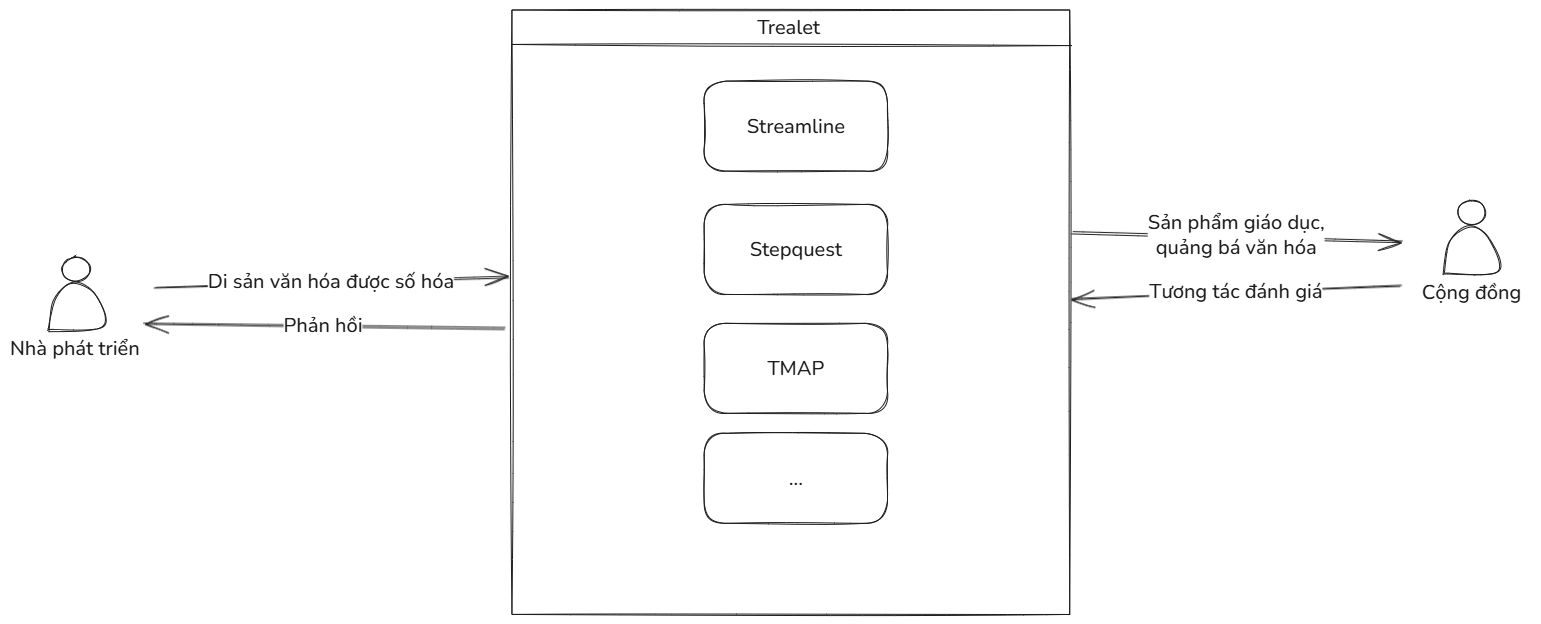
\includegraphics[width=0.8\textwidth]{figures/Hinh_Kien_Truc_Trealet.png}
    \caption{Tổng quan hệ thống Trealet và các ứng dụng con}
    \label{fig:trealet_overview}
\end{figure}

\section{Phân tích yêu cầu, đầu vào, đầu ra của TMAP}
\subsection{Phân tích yêu cầu}
TMAP hướng đến hai đối tượng người sử dụng là các nhà sáng tạo nội dung và
người trải nghiệm. Với các nhà sáng tạo nội dung, TMAP cung cấp một trình biên
soạn trên nển tảng Website, giúp các nhà sáng tạo dễ dàng truy cập với các thiết bị
Internet. Với đối tượng người trải nghiệm, TMAP cung cấp ứng dụng di động trên
nền tảng Android, tạo ra tính linh hoạt trong ứng dụng thực tế.
\subsection*{Yêu cầu chức năng}
Trình biên soạn cần cho phép các nhà sáng tạo nội dung có thể thêm, sửa,
xóa các bản đồ, các thao tác này cần được thực hiện thông qua các thao tác chọn lựa
đơn giản. Việc chọn các điểm tham quan cần cung cấp một bản đồ để nhà sáng tạo
có thể chọn vị trí thực tế, và nội dung của các điểm tham quan cần có khung đơn để
điền và tải lên các nội dung đa phương tiện. Các bản đồ sau khi được tạo và cập
nhật sẽ phải được lưu trong cơ sở dữ liệu.
Ứng dụng trải nghiệm cần cho phép người dùng xem danh sách bản đồ và
đáp ứng một bộ tìm kiếm để người dùng có thể tìm bản đò mình cần, đồng thời cần
có một màn hình để người dùng có thể trải nghiệm bản đồ mới hoặc xem lại các
phần tương tác với bản đồ đã lưu lại trước đó. Thông tin trải nghiệm này là thông
tin cá nhân cần được bảo mật, nên ứng dụng cũng cần đáp ứng việc xác thực người
dùng thông qua tạo tài khoản, đăng nhập, đăng xuất.
\subsection*{Yêu cầu phi chức năng}
Cả hai phần trình biên soạn và ứng dụng trải nghiệm cần phải có giao diện
thân thiện dễ dùng, riêng phần trải nghiệm cần có tổ chức giao diện hợp lý thu hút
người xem.
Phần biên tập nội dung cần phù hợp để được sử dụng bởi những người không
có chuyên môn sâu về công nghệ.

\subsection{Phân tích đầu vào, đầu ra của ứng dụng}
Đầu vào của trình biên soạn là thông tin về các địa điểm du lịch văn hóa bao
gồm vị trí, thông tin mô tả có thể bao gồm dữ liệu văn bản, đa phương tiện như ảnh,
video, đoạn audio và thứ tự lần lượt của các địa điểm đó. Đầu ra của trình biên soạn
sẽ là một đơn vị bản đồ được lưu trữ trong cơ sở dữ liệu lưu các thông tin của đầu ra
theo đúng trình tự, phục vụ cho ứng dụng trải nghiệm.
Đầu vào của ứng dụng trải nghiệm sẽ là danh sách các bản đồ đang có trên hệ
thống và thông tin người dùng. Dựa vào đầu vào này, ứng dụng trải nghiệm sẽ hiển
thị đầu ra là các bản đồ cho phép người dùng có thể trải nghiệm mới, hoặc xem lại
các phần tương tác đã được lưu trữ trước đó.

\section{Thiết kế}
\subsection{Thiết kế kiến trúc hệ thống}
Kiến trúc của TMAP sẽ phải có bốn phần, bên cạnh trình biên soạn và ứng
dụng trải nghiệm phải có một hệ thống server và cơ sở dữ liệu sẽ được sử dụng
chung. Server này sẽ đọc cơ sở dữ liệu và cung cấp thông tin các map, cho trình
biên soạn để thực hiện quản lý sửa xóa và cho ứng dụng trải nghiệm để dựng trải
nghiệm. Server cũng sẽ nhận thông tin bản đồ đã được cập nhật hoặc tạo mới từ
trình biên soạn để lưu lại vào trong cơ sở dữ liệu (\figurename~\ref{fig:tmap_design}).

\begin{figure}[h]
    \centering
    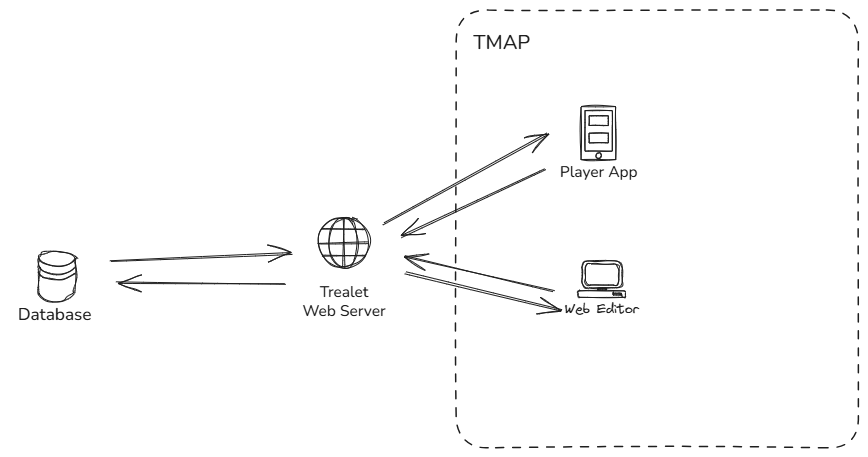
\includegraphics[width=0.8\textwidth]{figures/tmap_design.png}
    \caption{Kiến trúc hệ thống TMAP}
    \label{fig:tmap_design}
\end{figure}

Mỗi thành phần sẽ có kiến trúc kỹ thuật chi tiết như sau:
\begin{itemize}
\item Trình biên soạn sẽ là một trang Website được tích hợp vào trang quản lý
chung của TMAP, Website này sẽ cung cấp giao diện quản lý bản đồ cho
người dùng, và chuyển các thao tác quản lý thành các request để gửi cho
server xử lý. Sau khi nhận response từ server Website sẽ trình bày lại
phản hồi cho người dùng.
\item Ứng dụng trải nghiệm sẽ là một ứng dụng di động xây dựng cho nền tảng
Android, với giao diện để người dùng ban đầu có thể đăng nhập và lấy
thông tin về các bản đồ và trải nghiệm bản đồ sau đó. Các thao tác này
cũng sẽ được thực hiện thông qua các tương tác với server.
\item Server sẽ xử lý các yêu cầu của trình biên soạn và ứng dụng trải nghiệm,
và tùy thuộc vào các yêu cầu đó có thể truy xuất hoặc sửa đổi dữ liệu
trong cơ sở dữ liệu và trả lại phản hồi phù hợp.
\item Cơ sở dữ liệu sẽ là nơi lưu trữ thông tin về người dùng cũng như các bản
đồ đã được tạo ra, phục vụ cho Server xử lý các yêu cầu.
\end{itemize}

\subsection{Thiết kế luồng dữ liệu}
Tổng quan luồng dữ liệu của TMAP được mô tả trong \figurename~\ref{fig:tmap_dataflow}.

\begin{figure}[h]
    \centering
    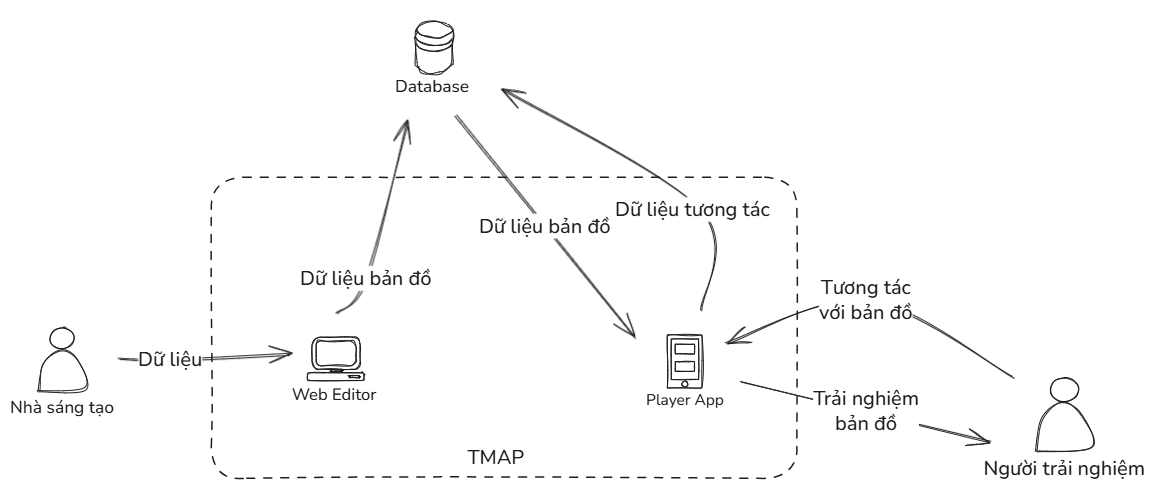
\includegraphics[width=0.8\textwidth]{figures/dataflow.png}
    \caption{Luồng dữ liệu của TMAP}
    \label{fig:tmap_dataflow}
\end{figure}

Trong luồng dữ liệu của Trình biên soạn, dữ liệu ban đầu sẽ là thông tin về các
điểm du lịch bao gồm vị trí, thông tin mô tả dưới dạng văn bản, ảnh, video, audio.
Trình biên soạn chuyển các thông tin này về dạng Map và tạo yêu cầu lưu trữ hoặc
sửa đổi để gửi về phía Server. Server nhận yêu cầu lưu trữ và lưu dữ liệu Bản đồ mới
vào Cơ sở dữ liệu.

Với luồng dữ liệu của Ứng dụng trải nghiệm, dữ liệu Bản đồ được Server trả
về theo yêu cầu được gửi từ ứng dụng, nó trình bày lại dữ liệu Bản đồ này dưới dạng một giao diện bản đồ. Thông qua tương tác với giao diện bản đồ này, người dùng có
thể thêm các tương tác của bản thân với điểm tham quan như chụp lại ảnh, ghi âm,
quét QR, gửi nội dung nhận xét bằng văn bản. Ứng dụng trải nghiệm nhận các tương
tác này và gửi yêu cầu lưu tương tác để Server có thể lưu hoặc cập nhật tương tác vào
phần thông tin trải nghiệm của người dùng đối với Bản đồ.

\subsection{Thiết kế cơ sở dữ liệu}
TMAP sử dụng chung cơ sở dữ liệu với hệ thống chung Trealet, với các tác vụ được thực hiện tập trung trên 3 bảng au\_trealets, au\_users và au\_user\_to\_trealet.
Bảng au\_trealets lưu thông tin các bản đồ, au\_users lưu thông tin người dùng, và
au\_user\_to\_trealet lưu thông tin các tương tác của người dùng với bản đồ. Mối quan
hệ giữa các bảng được miêu tả trong \figurename~\ref{fig:tmap_database}.


\begin{figure}[h]
    \centering
    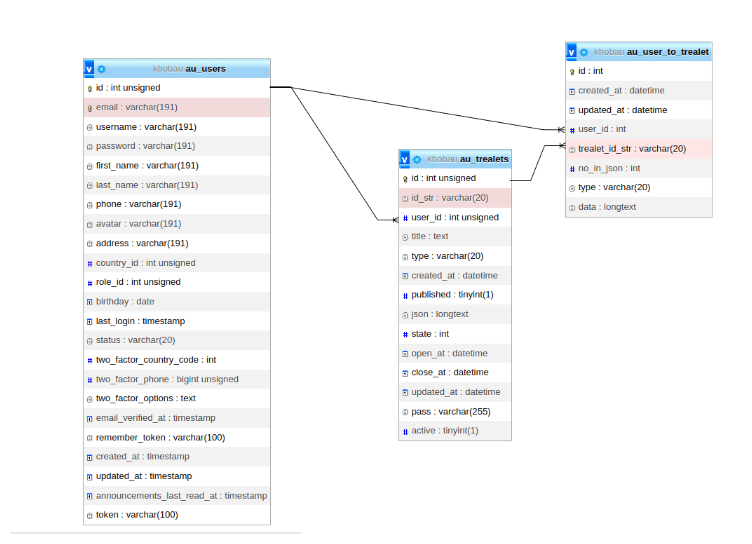
\includegraphics[width=0.8\textwidth]{figures/erd.png}
    \caption{Mối quan hệ giữa các bảng trong cơ sở dữ liệu TMAP}
    \label{fig:tmap_database}
\end{figure}

\subsection{Thiết kế ứng dụng}
\subsection*{Phân tích hệ thống}
Các khái niệm chính:
\begin{itemize}
    \item \textbf{Người dùng}: Một đơn vị người dùng của được định danh bằng một tài khoản trong
hệ thống
    \item \textbf{Bản đồ}: Bản đồ trải nghiệm được tạo ra từ Trình biên soạn, được trải nghiệm
bằng cách sử dụng Ứng dụng trải nghiệm và được lưu trong cơ sở dữ liệu cùng với
các thành phần khác của Trealet, với sự khác biệt ở trường dữ liệu json
    \item \textbf{Tương tác}: Một tương tác được Người dùng tạo ra khi trải nghiệm Bản đồ, được lưu
trong bảng au\_user\_to\_trealet.
\end{itemize}
Các tác nhân chính:
\begin{itemize}
    \item \textbf{Quản trị viên}: Người dùng với quyền hạn cao nhất, quản lý toàn bộ hệ thống bao gồm người dùng, bản đồ, các tương tác.
    \item \textbf{Người sáng tạo}: Người dùng sáng tạo, có thể tạo ra các bản đồ và quản lý các bản đồ mình tạo ra.
    \item \textbf{Người trải nghiệm}: Người dùng trải nghiệm, có thể tạo ra tương tác trên các bản đồ thông qua việc trải nghiệm bản đồ, và xem lại các trải nghiệm này thông qua Ứng dụng trải nghiệm.
\end{itemize}

\subsection*{Mô tả ca sử dụng}
Dựa trên các khái niệm và tác nhân trên, hệ thống có các ca sử dụng sau:

\textbf{Ca sử dụng của Quản trị viên}

Quản trị viên sẽ là tài khoản Người dùng được tạo trước, có thể đăng nhập và thực hiện thao
tác Thêm, Sửa, Xóa với cả hai tài nguyên là người dùng và Bản đồ (\figurename~\ref{fig:admin_use_case}).
\begin{figure}[h]
    \centering
    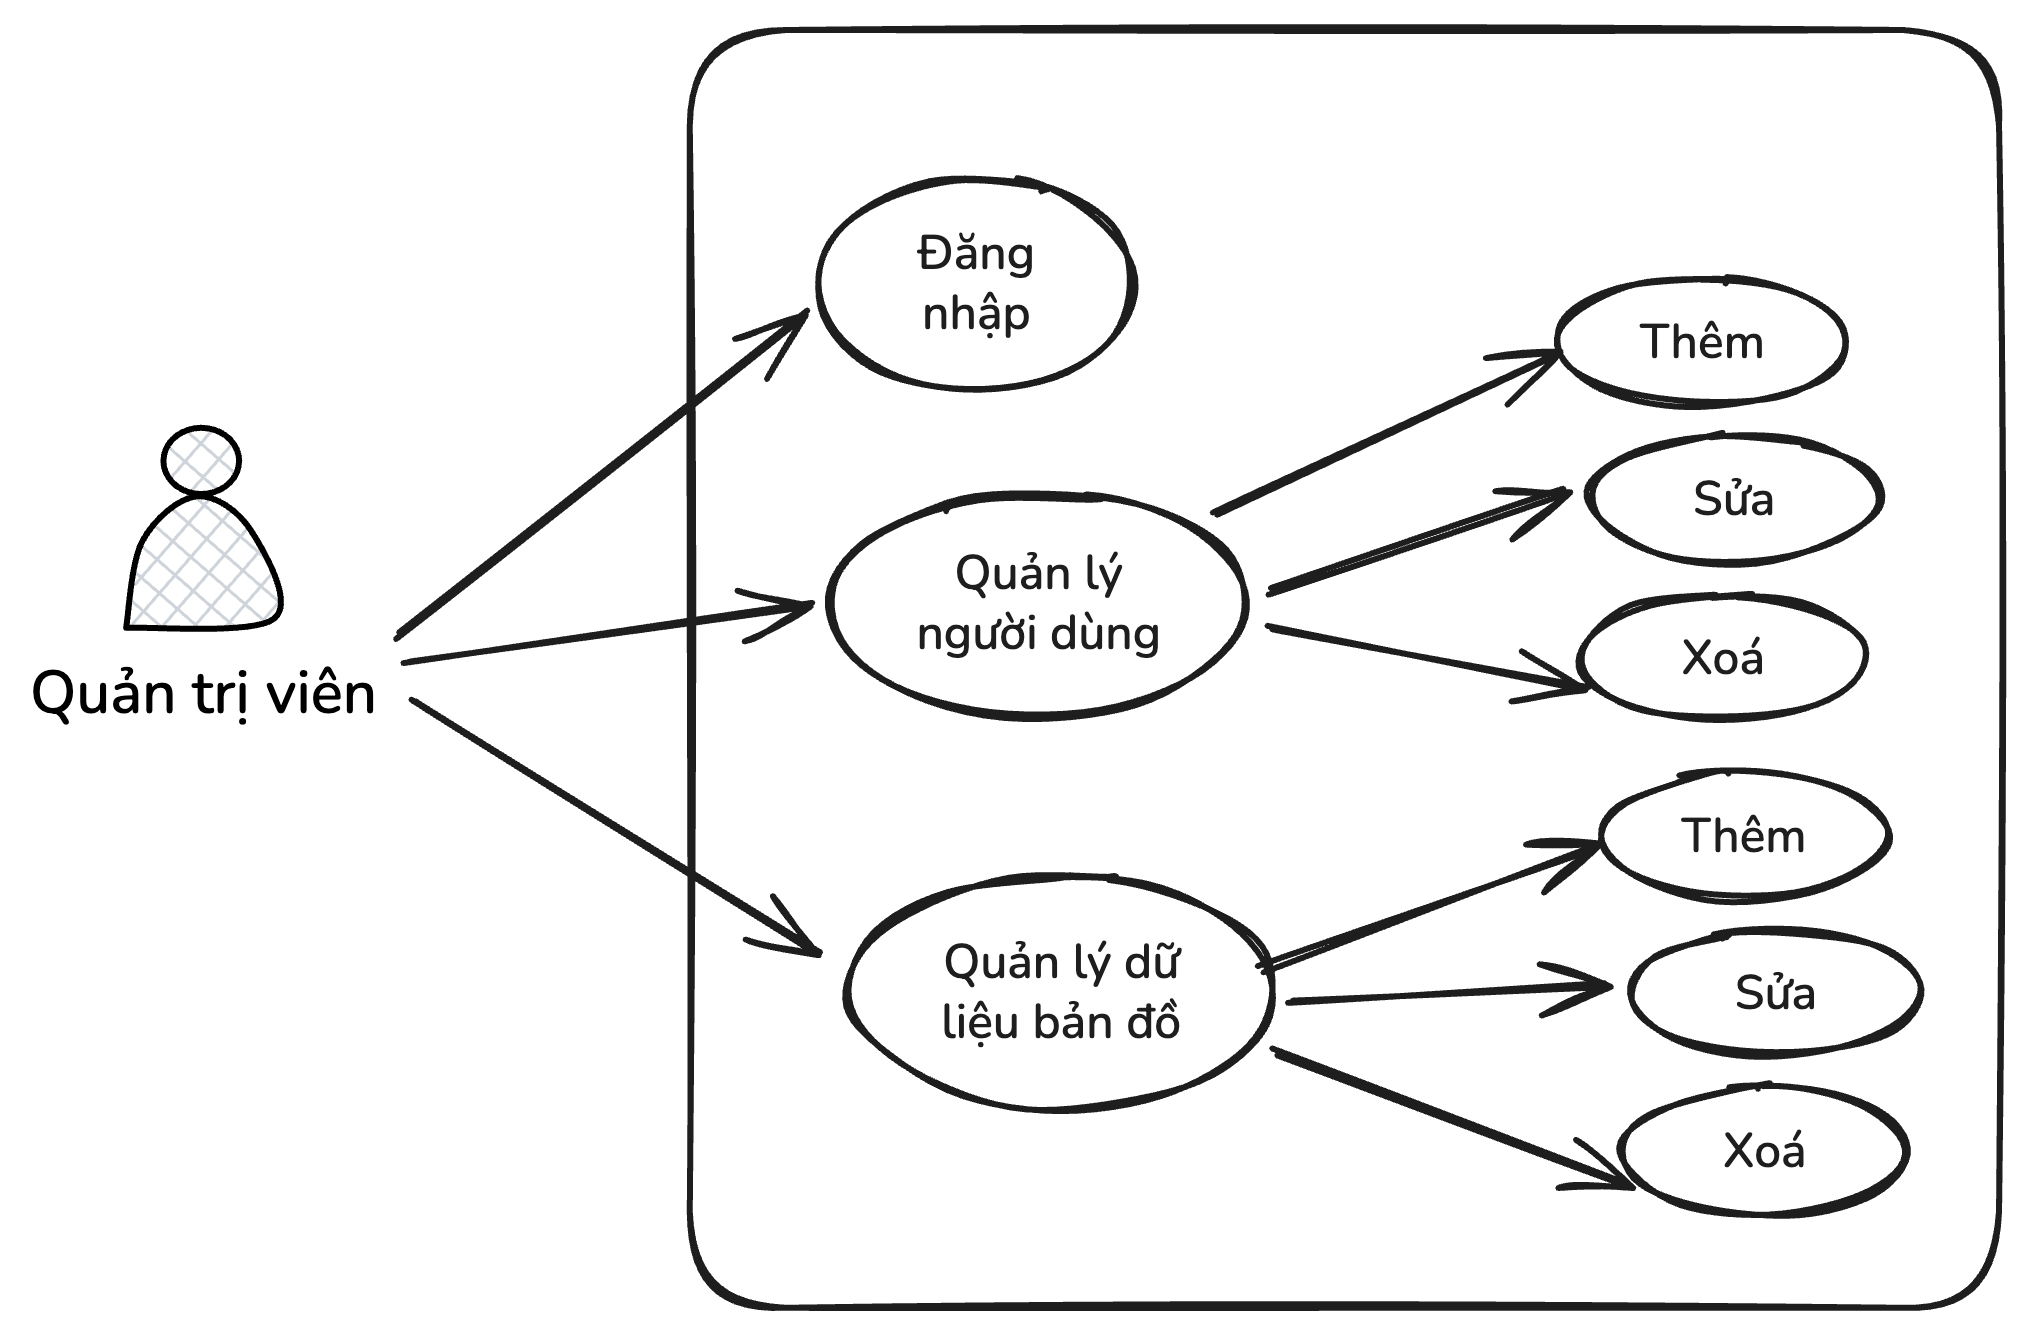
\includegraphics[width=0.6\textwidth]{figures/admin-use-case.excalidraw.png}
    \caption{Ca sử dụng của Quản trị viên}
    \label{fig:admin_use_case}
\end{figure}

\textbf{Ca sử dụng của Người sáng tạo}

Nhà sáng tạo nội dung sẽ có các ca sử dụng như đăng ký, đăng nhập, cập nhật
thông tin người dùng, Thêm, Sửa, Xóa các Bản đồ mà mình tạo ra qua Trình biên soạn,
đồng thời cũng có thể trải nghiệm toàn bộ các Bản đồ thông qua Ứng dụng trải nghiệm
(\figurename~\ref{fig:creator_use_case}).
\begin{figure}[h]
    \centering
    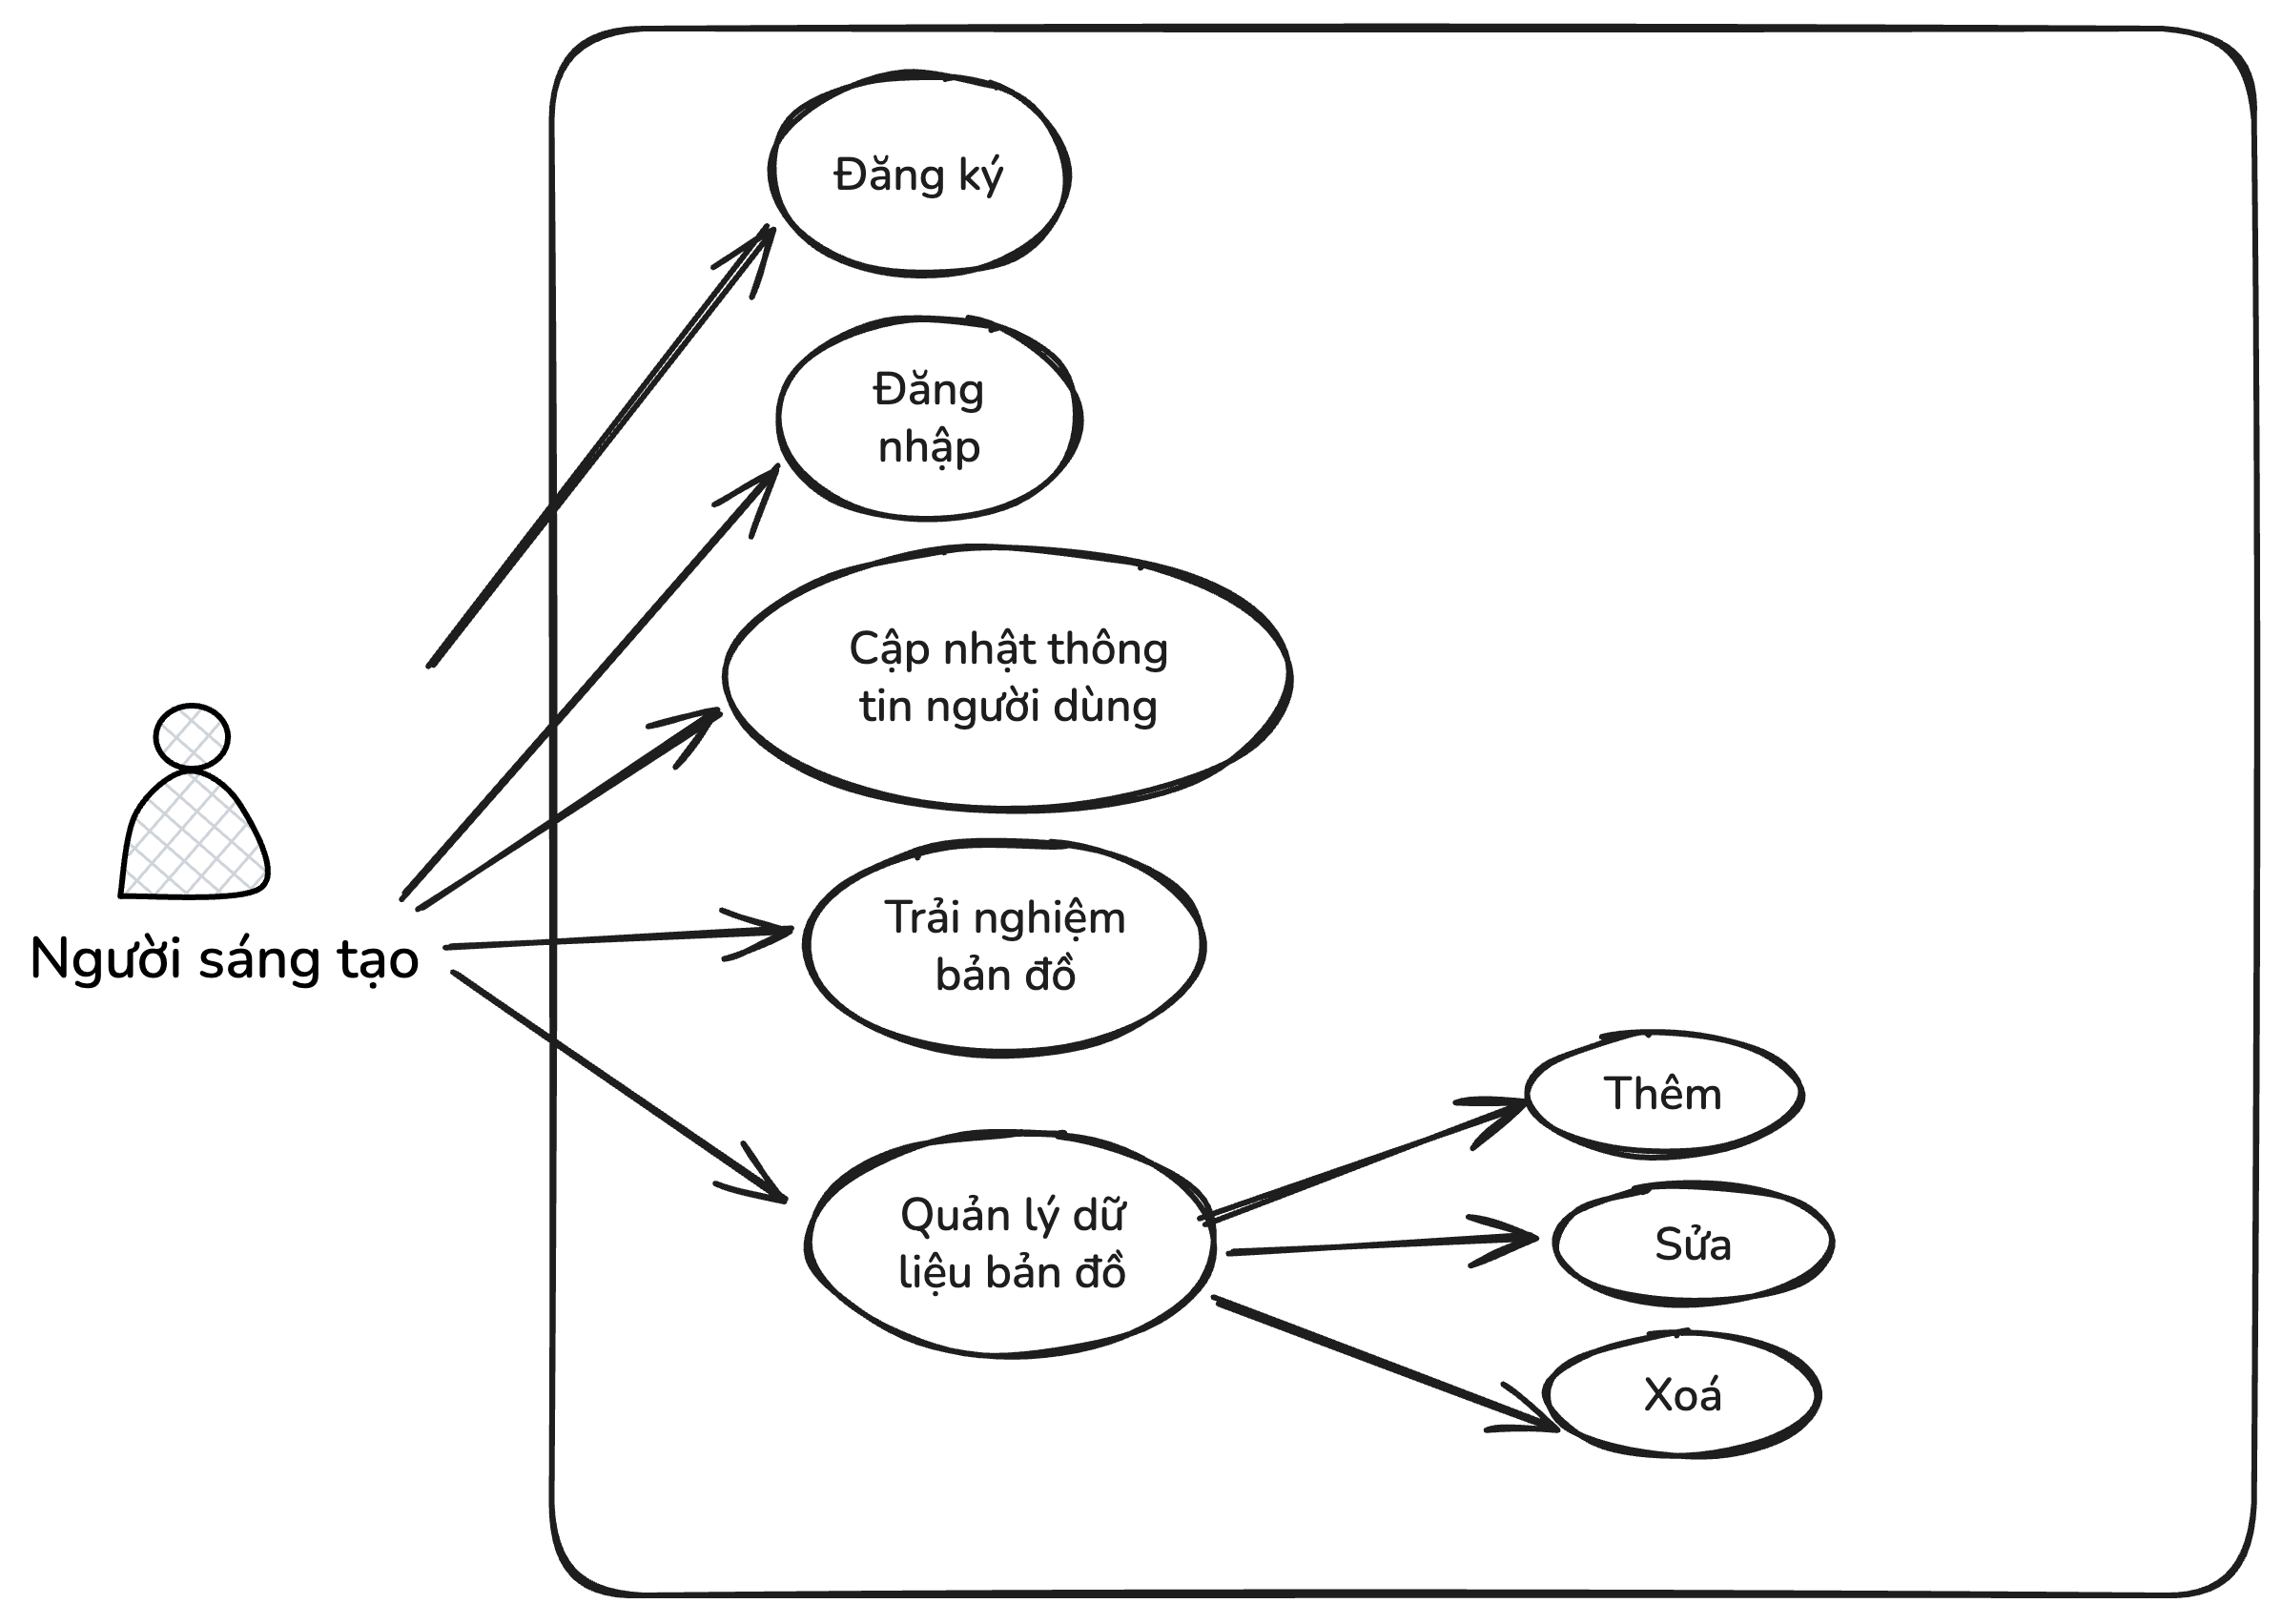
\includegraphics[width=0.8\textwidth]{figures/creator-use-case.excalidraw.png}
    \caption{Ca sử dụng của Người sáng tạo}
    \label{fig:creator_use_case}
\end{figure}

\textbf{Ca sử dụng của Người trải nghiệm}

Người trải nghiệm có thể đăng nhập, đăng ký, sửa đổi thông tin tài khoản và
trải nghiệm các Bản đồ thông qua Ứng dụng trải nghiệm (\figurename~\ref{fig:user_use_case}).
\begin{figure}[h]
    \centering
    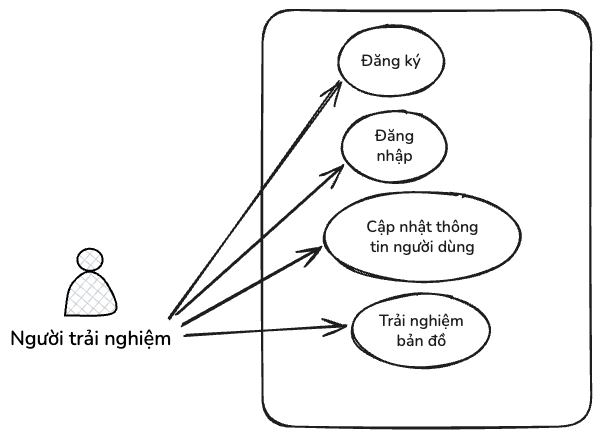
\includegraphics[width=0.8\textwidth]{figures/user-use-case.excalidraw.png}
    \caption{Ca sử dụng của Người trải nghiệm}
    \label{fig:user_use_case}
\end{figure}


\subsection*{Mô tả chi tiết ca sử dụng}
Các ca sử dụng trong hệ thống sẽ được mô tả chi tiết trong các bảng:

\begin{table}
\centering
\caption{Phân tích ca sử dụng đăng nhập bằng tài khoản mật khẩu}
\begin{tabular}{|p{4cm}|p{10cm}|}
\hline
\textbf{Mô tả} & Đăng nhập bằng tài khoản mật khẩu \\ \hline
\textbf{Tác nhân} & Quản trị viên, Người sáng tạo, Người trải nghiệm \\ \hline
\textbf{Điều kiện ban đầu} & Tài khoản người dùng đã tồn tại trên hệ thống \\ \hline
\textbf{Điều kiện sau} & 
\textbf{Thành công:} Trình biên soạn thông báo người dùng đăng nhập thành công, chuyển người dùng tới trang chủ. Ứng dụng trải nghiệm chuyển người dùng tới màn hình danh sách Map để trải nghiệm. \\
& \textbf{Thất bại:} Hiển thị lỗi cho người dùng. \\ \hline
\textbf{Luồng sự kiện chính} & 
1. Người dùng truy cập vào hệ thống, chọn nút đăng nhập. \newline
2. Hệ thống hiển thị giao diện đăng nhập. \newline
3. Người dùng nhập thông tin đăng nhập (email và mật khẩu) và ấn đăng nhập. \newline
4. Hệ thống kiểm tra xác thực người dùng và trả về kết quả tương ứng. \\ \hline
\textbf{Luồng ngoại lệ} & Khi người dùng nhập sai thông tin tài khoản hoặc thông tin không tồn tại, hệ thống hiển thị thông báo lỗi và trả người dùng về màn hình đăng nhập. \\ \hline
\textbf{Yêu cầu đặc biệt} & Không \\ \hline
\textbf{Mở rộng} & Không \\ \hline
\end{tabular}
\end{table}

\begin{table}
\centering
\caption{Phân tích ca sử dụng đăng nhập bằng tài khoản Google}
\begin{tabular}{|p{4cm}|p{10cm}|}
    \hline
\textbf{Mô tả} & Đăng nhập bằng tài khoản Google \\ \hline
\textbf{Tác nhân} & Quản trị viên, Người sáng tạo, Người trải nghiệm \\ \hline
\textbf{Điều kiện ban đầu} & Không \\ \hline
\textbf{Điều kiện sau} & Hệ thống tạo mới tài khoản với email Google đã đăng nhập nếu chưa tồn tại tài khoản với email đó trong hệ thống \\ \hline
\textbf{Luồng sự kiện chính} & 
1. Người dùng truy cập vào hệ thống, chọn nút đăng nhập bằng Google \newline
2. Hệ thống chuyển hướng người dùng tới trang đăng nhập với Google \newline
3. Người dùng đăng nhập với tài khoản Google \newline
4. Hệ thống nhận kết quả xác thực từ Google và phản hồi \\ \hline
\textbf{Luồng ngoại lệ} & Không \\ \hline
\textbf{Yêu cầu đặc biệt} & Không \\ \hline
\textbf{Mở rộng} & Không \\ \hline
\end{tabular}
\end{table}

\begin{table}
\centering
\caption{Phân tích ca sử dụng đặt lại mật khẩu}
\begin{tabular}{|p{4cm}|p{10cm}|}
    \hline
\textbf{Mô tả} & Đặt lại mật khẩu \\ \hline
\textbf{Tác nhân} & Quản trị viên, Người sáng tạo, Người trải nghiệm \\ \hline
\textbf{Điều kiện ban đầu} & Tài khoản người dùng đã tồn tại trên hệ thống \\ \hline
\textbf{Điều kiện sau} & Hệ thống gửi email với mật khẩu đã đặt lại cho vào tài khoản email của người dùng \\ \hline
\textbf{Luồng sự kiện chính} & 
1. Người dùng truy cập vào hệ thống, chọn nút đăng nhập \newline
2. Hệ thống hiển thị giao diện đăng nhập \newline
3. Người dùng chọn vào phần quên mật khẩu \newline
4. Hệ thống hiển thị khung nhập email cho người dùng \newline
5. Người dùng nhập email và chọn đặt lại mật khẩu \newline
6. Hệ thống xác thực email và gửi mật khẩu đã đặt lại vào email nếu đúng \\ \hline
\textbf{Luồng ngoại lệ} & Không \\ \hline
\textbf{Yêu cầu đặc biệt} & Không \\ \hline
\textbf{Mở rộng} & Không \\ \hline
\end{tabular}
\end{table}

\begin{table}
\centering
\caption{Phân tích ca sử dụng đăng ký}
\begin{tabular}{|p{4cm}|p{10cm}|}
    \hline
\textbf{Mô tả} & Đăng ký tài khoản \\ \hline
\textbf{Tác nhân} & Quản trị viên, Người sáng tạo, Người trải nghiệm \\ \hline
\textbf{Điều kiện ban đầu} & Tài khoản người dùng chưa tồn tại \\ \hline
\textbf{Điều kiện sau} & \textbf{Thành công:} Trình biên soạn thông báo người dùng đăng ký thành công, chuyển  
người dùng tới trang chủ. Ứng dụng trải
nghiệm chuyển người dùng tới màn hình
chính để đăng nhập. Hệ thống tạo ra và
lưu tài khoản mới. \newline
\textbf{Thất bại:} Hiển thị lỗi cho người dùng \\ \hline
\textbf{Luồng sự kiện chính} &
1. Người dùng truy cập vào hệ
thống, chọn nút đăng ký \newline
2. Hệ thống hiển thị giao diện đăng
ký \newline
3. Người dùng nhập thông tin đăng
ký bao gồm email, tên tài khoản
và mật khẩu, ấn đăng ký \newline
4. Hệ thống kiểm tra xem đã tồn tại
thông tin tài khoản chưa và phản
hồi \newline \\ \hline
\textbf{Luồng ngoại lệ} & Khi người dùng nhập sai quy định về thông tin tài khoản hoặc nhập thông tin tài khoản đã tồn tại trong hệ thống, hệ thống sẽ đưa ra thông báo lỗi và đưa người dùng trở lại màn hình đăng ký để nhập lại thông tin. \\ \hline
\textbf{Yêu cầu đặc biệt} & Không \\ \hline
\textbf{Mở rộng} & Không \\ \hline
\end{tabular}
\end{table}

\begin{table}
\centering
\caption{Phân tích ca sử dụng cập nhật mật khẩu}
\begin{tabular}{|p{4cm}|p{10cm}|}
    \hline
\textbf{Mô tả} & Cập nhật mật khẩu \\ \hline
\textbf{Tác nhân} & Quản trị viên, Người sáng tạo, Người trải nghiệm \\ \hline
\textbf{Điều kiện ban đầu} & Người dùng đã đăng nhập vào hệ thống \\ \hline
\textbf{Điều kiện sau} & 
\textbf{Thành công:} Hệ thống thông báo người dùng thay đổi mật khẩu thành công. Chuyển người dùng đến trang đăng nhập để đăng nhập lại \newline
\textbf{Thất bại:} Hiển thị lỗi cho người dùng \\ \hline
\textbf{Luồng sự kiện chính} & 
1. Người dùng chọn phần quản lý
tài khoản trên giao diện \newline
2. Hệ thống hiển thị giao diện quản
lý tài khoản \newline
3. Người dùng chọn cập nhật mật
khẩu, nhập lại mật khẩu cũ và mật
khẩu mới \newline
4. Hệ thống kiểm tra xác thực mật
khẩu cũ, cập nhật mật khẩu nếu
thành công \\ \hline
\textbf{Luồng ngoại lệ} & Khi người dùng nhập sai thông tin mật khẩu, yêu cầu sửa mật khẩu sẽ bị hủy và hệ thống sẽ báo lỗi. \\ \hline
\textbf{Yêu cầu đặc biệt} & Không \\ \hline
\textbf{Mở rộng} & Không \\ \hline
\end{tabular}
\end{table}
\begin{table}
\centering
\caption{Phân tích ca sử dụng cập nhật thông tin người dùng}
\begin{tabular}{|p{4cm}|p{10cm}|}
    \hline
\textbf{Mô tả} & Cập nhật thông tin người dùng \\ \hline
\textbf{Tác nhân} & Quản trị viên, Người sáng tạo, Người trải nghiệm \\ \hline
\textbf{Điều kiện ban đầu} & Người dùng đã đăng nhập vào hệ thống \\ \hline
\textbf{Điều kiện sau} & 
\textbf{Thành công:} Hệ thống cập nhật lại thông tin người dùng. \newline
\textbf{Thất bại:} Hiển thị lỗi cho người dùng \\ \hline
\textbf{Luồng sự kiện chính} & 
1. Người dùng chọn phần quản lý
tài khoản trên giao diện \newline
2. Hệ thống hiển thị giao diện quản
lý tài khoản \newline
3. Người dùng chọn sửa đổi và thực
hiện cập nhật các thông tin và ấn
cập nhật. \newline
4. Hệ thống kiểm tra các thông tin
xem đã đúng định dạng hay chưa,
và phản hồi tương ứng \\ \hline
\textbf{Luồng ngoại lệ} & Khi người dùng nhập thông tin sai định dạng, hệ thống trả lại lỗi cho người dùng để thông báo. \\ \hline
\textbf{Yêu cầu đặc biệt} & Không \\ \hline
\textbf{Mở rộng} & Không \\ \hline
\end{tabular}
\end{table}

\begin{table}
\centering
\caption{Phân tích ca sử dụng đăng xuất}
\begin{tabular}{|p{4cm}|p{10cm}|}
    \hline
\textbf{Mô tả} & Đăng xuất \\ \hline
\textbf{Tác nhân} & Quản trị viên, Người sáng tạo, Người trải nghiệm \\ \hline
\textbf{Điều kiện ban đầu} & Người dùng đã đăng nhập vào hệ thống \\ \hline
\textbf{Điều kiện sau} & Hệ thống đăng xuất người dùng. Trình biên soạn trả người dùng về trang chủ, Ứng dụng trải nghiệm trả người dùng về trang đăng nhập. \\ \hline
\textbf{Luồng sự kiện chính} & 
1. Người dùng chọn đăng xuất trên
giao diện \newline
2. Hệ thống đăng xuất người dùng,
trả người dùng về trang tương
ứng \\ \hline
\textbf{Luồng ngoại lệ} & Không \\ \hline
\textbf{Yêu cầu đặc biệt} & Không \\ \hline
\textbf{Mở rộng} & Không \\ \hline
\end{tabular}
\end{table}
\begin{table}
\centering
\caption{Phân tích ca sử dụng tạo Map}
\begin{tabular}{|p{4cm}|p{10cm}|}
    \hline
\textbf{Mô tả} & Ca sử dụng tạo Bản đồ \\ \hline
\textbf{Tác nhân} & Quản trị viên, Người sáng tạo \\ \hline
\textbf{Điều kiện ban đầu} & Người dùng đã đăng nhập vào hệ thống \\ \hline
\textbf{Điều kiện sau} & 
\textbf{Thành công:} Hệ thống tạo ra Bản đồ mới và lưu vào cơ sở dữ liệu. \newline
\textbf{Thất bại:} Hiển thị lỗi cho người dùng \\ \hline
\textbf{Luồng sự kiện chính} & 
1. Người dùng chọn phần quản lý
Trealet trên giao diện, và chọn
phần Map \newline
2. Hệ thống hiển thị màn hình danh
sách Bản đồ của người dùng \newline
3. Người dùng chọn new map \newline
4. Hệ thống hiển thị ra Trình
biên soạn \newline
5. Người dùng nhập các thông tin
mô tả cho Bản đồ, bao gồm các vị
trí trải nghiệm, mô tả và tương tác
của các vị trí, định danh của Bản
đồ \newline
6. Hệ thống kiểm tra thông tin của
Bản đồ đã phù hợp theo quy định
hay chưa và phản hồi tương ứng \\ \hline
\textbf{Luồng ngoại lệ} & Khi người dùng nhập thông tin sai định dạng, hệ thống trả lại lỗi cho người dùng để thông báo \\ \hline
\textbf{Yêu cầu đặc biệt} & Không \\ \hline
\textbf{Mở rộng} & Không \\ \hline
\end{tabular}
\end{table}

\begin{table}
\centering
\caption{Phân tích ca sử dụng cập nhật Bản đồ}
\begin{tabular}{|p{4cm}|p{10cm}|}
    \hline
\textbf{Mô tả} & Ca sử dụng cập nhật Bản đồ \\ \hline
\textbf{Tác nhân} & Quản trị viên, Người sáng tạo \\ \hline
\textbf{Điều kiện ban đầu} & Người dùng đã đăng nhập vào hệ thống \\ \hline
\textbf{Điều kiện sau} & 
\textbf{Thành công:} Hệ thống cập nhật lại thông tin của Bản đồ. \newline
\textbf{Thất bại:} Hiển thị lỗi cho người dùng \\ \hline
\textbf{Luồng sự kiện chính} & 
1. Người dùng chọn phần quản lý
Trealet trên giao diện, và chọn
phần Bản đồ \newline
2. Hệ thống hiển thị màn hình danh
sách Bản đồ của người dùng \newline
3. Người dùng chọn nút sửa đổi trên
Bản đồ cần sửa đổi. \newline
4. Hệ thống chuyển người dùng đến
Trình biên soạn có chứa thông tin
của Bản đồ đó \newline
5. Người dùng cập nhật các thông
tin mô tả cho Bản đồ, bao gồm các vị
trí trải nghiệm, mô tả và tương tác
của các vị trí, định danh của Bản
đồ \newline
6. Hệ thống kiểm tra các thông tin
xem đã đúng định dạng hay chưa,
và phản hồi tương ứng \\ \hline
\textbf{Luồng ngoại lệ} & Khi người dùng nhập thông tin sai định dạng, hệ thống trả lại lỗi cho người dùng để thông báo \\ \hline
\textbf{Yêu cầu đặc biệt} & Không \\ \hline
\textbf{Mở rộng} & Không \\ \hline
\end{tabular}
\end{table}
\begin{table}
\centering
\caption{Phân tích ca sử dụng xóa Bản đồ}
\begin{tabular}{|p{4cm}|p{10cm}|}
    \hline
\textbf{Mô tả} & Ca sử dụng xóa Bản đồ \\ \hline
\textbf{Tác nhân} & Quản trị viên, Người sáng tạo \\ \hline
\textbf{Điều kiện ban đầu} & Người dùng đã đăng nhập vào hệ thống \\ \hline
\textbf{Điều kiện sau} & Hệ thống xóa đi Bản đồ người dùng đã chọn \\ \hline
\textbf{Luồng sự kiện chính} & 
1. Người dùng chọn phần quản lý
Trealet trên giao diện, và chọn
phần Map \newline
2. Hệ thống hiển thị màn hình danh
sách Bản đồ của người dùng \newline
3. Người dùng chọn nút xóa trên
Bản đồ cần xóa. \newline
4. Hệ thống hiển thị thông báo để
người dùng xác nhận xóa Bản đồ \newline
5. Người dùng ấn xác nhận để xóa
Bản đồ, ấn hủy để hủy. \\ \hline
\textbf{Luồng ngoại lệ} & Không \\ \hline
\textbf{Yêu cầu đặc biệt} & Không \\ \hline
\textbf{Mở rộng} & Không \\ \hline
\end{tabular}
\end{table}
\begin{table}
\centering
\caption{Phân tích ca sử dụng xem danh sách Bản đồ trải nghiệm}
\begin{tabular}{|p{4cm}|p{10cm}|}
    \hline
\textbf{Mô tả} & Ca sử dụng xem danh sách Bản đồ trải nghiệm \\ \hline
\textbf{Tác nhân} & Quản trị viên, Người sáng tạo, Người trải nghiệm \\ \hline
\textbf{Điều kiện ban đầu} & Người dùng đã đăng nhập vào hệ thống \\ \hline
\textbf{Điều kiện sau} & Ứng dụng trải nghiệm hiển thị màn hình trải nghiệm \\ \hline
\textbf{Luồng sự kiện chính} & 
1. Hệ thống hiển thi danh sách Bản đồ
cùng với một thanh tìm kiếm sau
khi người dùng đã đăng nhập
thành công vào Ứng dụng trải
nghiệm \newline
2. Người dùng tìm kiếm Bản đồ bằng
thanh tìm kiếm và chọn Bản đồ
người dùng muốn trải nghiệm \newline
3. Hệ thống trả lại màn hình trải
nghiệm với Bản đồ tương ứng \\ \hline
\textbf{Luồng ngoại lệ} & Không \\ \hline
\textbf{Yêu cầu đặc biệt} & Không \\ \hline
\textbf{Mở rộng} & Không \\ \hline
\end{tabular}
\end{table}
\begin{table}
\centering
\caption{Phân tích ca sử dụng thêm tương tác khi trải nghiệm Bản đồ}
\begin{tabular}{|p{4cm}|p{10cm}|}
    \hline
\textbf{Mô tả} & Ca sử dụng thêm tương tác khi trải nghiệm Bản đồ \\ \hline
\textbf{Tác nhân} & Quản trị viên, Người sáng tạo, Người trải nghiệm \\ \hline
\textbf{Điều kiện ban đầu} & Người dùng đã hoàn thành ca sử dụng trải nghiệm Bản đồ \\ \hline
\textbf{Điều kiện sau} & Ứng dụng trải nghiệm cập nhật tương tác của người dùng với điểm tham quan lên hệ thống chung \\ \hline
\textbf{Luồng sự kiện chính} & 
1. Người dùng chọn điểm tham quan thông qua màn hình trải nghiệm. \newline
2. Ứng dụng trải nghiệm hiển thị khung mô tả địa điểm và tương tác địa điểm \newline
3. Người dùng chọn phần tương tác và thực hiện tương tác tương ứng, ấn nút lưu khi thực hiện xong. \newline
4. Hệ thống lưu lại tương tác đó, cập
nhật rằng người dùng đã hoàn
thành điểm tham quan và trả về
thông báo thành công \\ \hline
\textbf{Luồng ngoại lệ} & Không \\ \hline
\textbf{Yêu cầu đặc biệt} & Không \\ \hline
\textbf{Mở rộng} & Không \\ \hline
\end{tabular}
\end{table}
\begin{table}
\centering
\caption{Phân tích ca sử dụng cập nhật tương tác trên Bản đồ đã trải nghiệm}
\begin{tabular}{|p{4cm}|p{10cm}|}
    \hline
\textbf{Mô tả} & Ca sử dụng cập nhật tương tác trên Bản đồ đã trải nghiệm \\ \hline
\textbf{Tác nhân} & Quản trị viên, Người sáng tạo, Người trải nghiệm \\ \hline
\textbf{Điều kiện ban đầu} & Người dùng đã hoàn thành ca sử dụng trải nghiệm Bản đồ \\ \hline
\textbf{Điều kiện sau} & Ứng dụng trải nghiệm cập nhật lại tương tác của người dùng với điểm tham quan lên hệ thống \\ \hline
\textbf{Luồng sự kiện chính} & 1. Người dùng chọn điểm tham quan đã tương tác trước đó thông qua màn hình trải nghiệm. \newline
2. Ứng dụng trải nghiệm hiển thị khung mô tả địa điểm và tương tác địa điểm. \newline
3. Người dùng chọn phần tương tác và ấn cập nhật, thực hiện tương tác tương ứng, ấn nút lưu khi thực hiện xong. \newline
4. Hệ thống lưu lại tương tác đó, cập nhật rằng người dùng đã hoàn thành điểm tham quan và trả về thông báo thành công. \\ \hline
\textbf{Luồng ngoại lệ} & Không \\ \hline
\textbf{Yêu cầu đặc biệt} & Không \\ \hline
\textbf{Mở rộng} & Không \\ \hline
\end{tabular}
\end{table}

\newpage
\subsection{Thiết kế giao diện}
\textbf{Trình biên soạn}

Người dùng truy cập giao diện chung của Trình biên soạn để quản lý các Bản đồ,
hoặc tạo Bản đồ mới (\figurename~\ref{fig:editor-main}). Giao diện tạo Bản đồ mới và sửa Bản đồ được chia làm hai
phần, thông tin chung của Bản đồ và thông tin chi tiết cho từng địa điểm. Người dùng
sẽ bắt đầu bằng việc hoàn thiện phần thông tin chung của Bản đồ, bao gồm tiêu đề, mô
tả về bản đồ, trạng thái phát hành (\figurename~\ref{fig:editor-map-info}). Ở trạng thái phát hành có mật khẩu, giao
diện sẽ cung cấp một khung nhập mật khẩu cho người dùng (\figurename~\ref{fig:editor-map-password}). Trong giao
diện điền chi tiết các điểm tham quan, người biên soạn sẽ có các khung để nhập tiêu
đề, mô tả bằng văn bản, nút đăng tải nội dung đa phương tiện, khung chọn hình thức
tương tác và mô tả tương tác (\figurename~\ref{fig:editor-point-info}).

\begin{figure}[h]
    \centering
    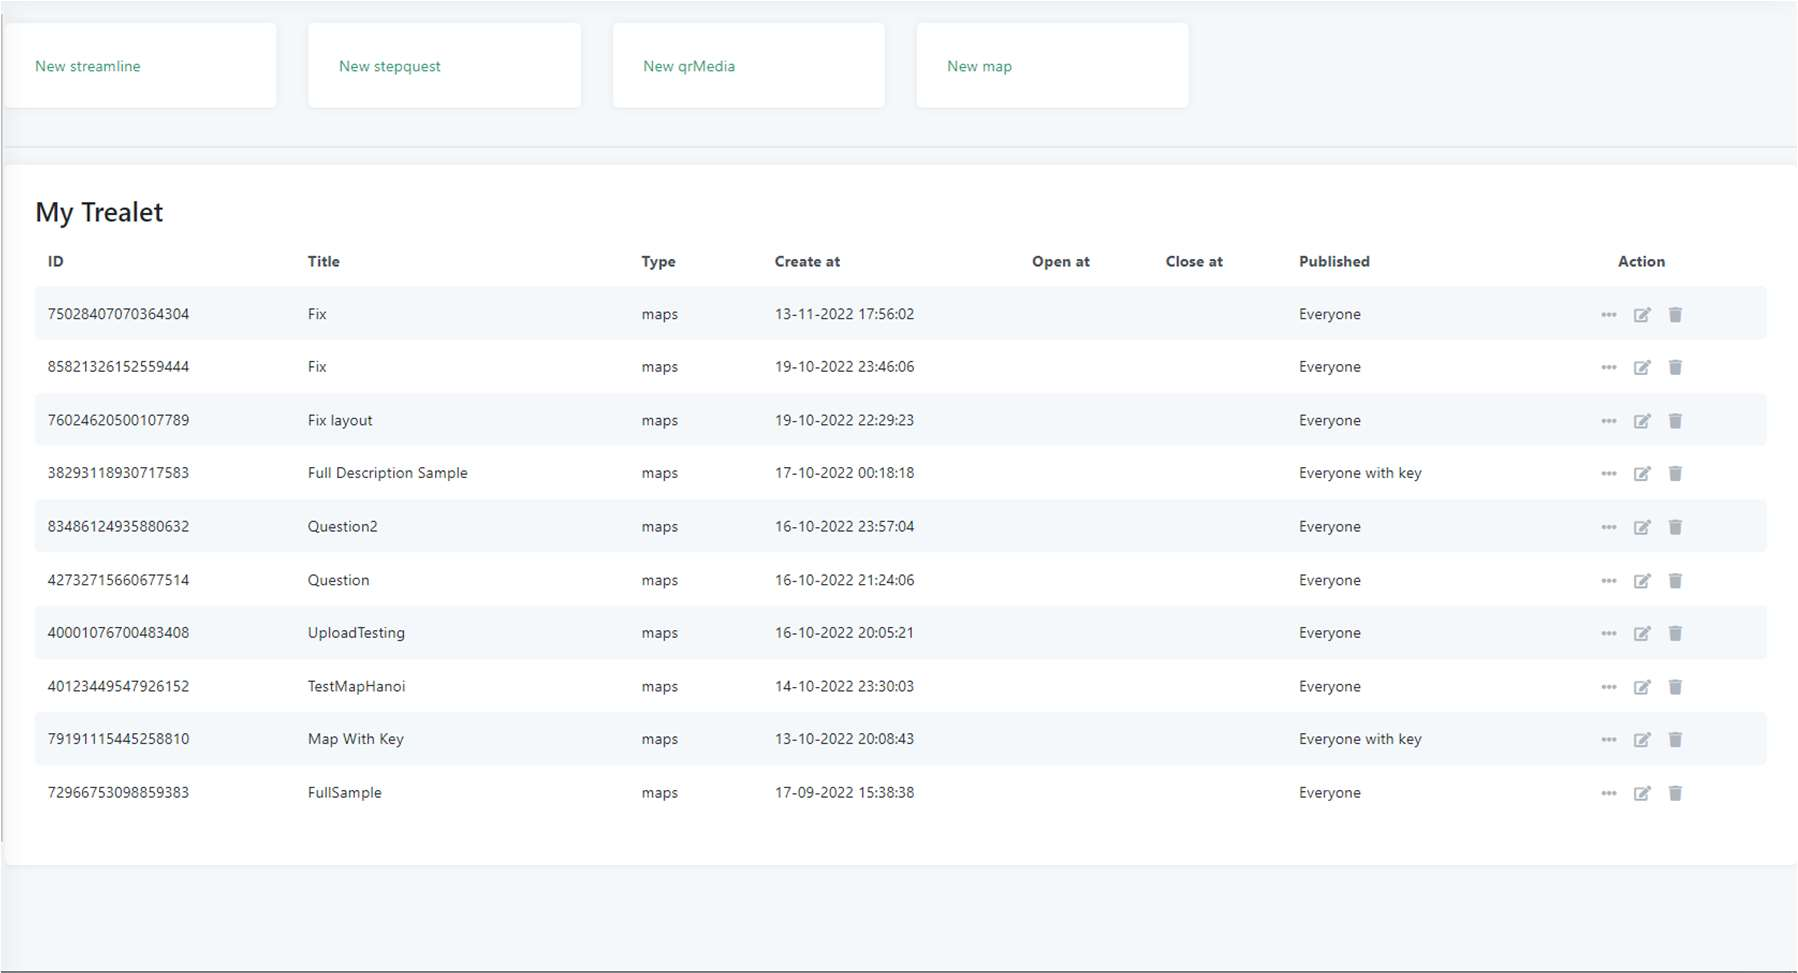
\includegraphics[width=0.8\textwidth]{figures/editor-main.jpg}
    \caption{Giao diện chính của Trình biên soạn}
    \label{fig:editor-main}
\end{figure}

\begin{figure}[h]
    \centering
    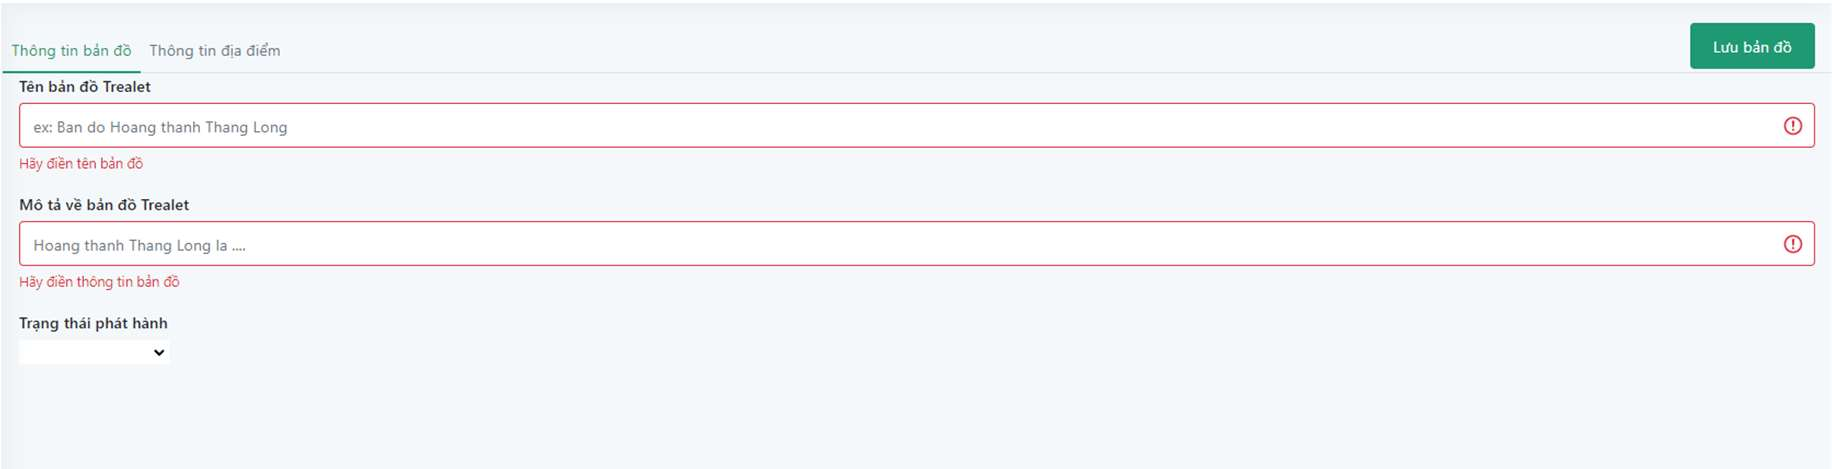
\includegraphics[width=0.8\textwidth]{figures/editor-map-info.jpg}
    \caption{Giao diện nhập thông tin chung của Bản đồ}
    \label{fig:editor-map-info}
\end{figure}

\begin{figure}[h]
    \centering
    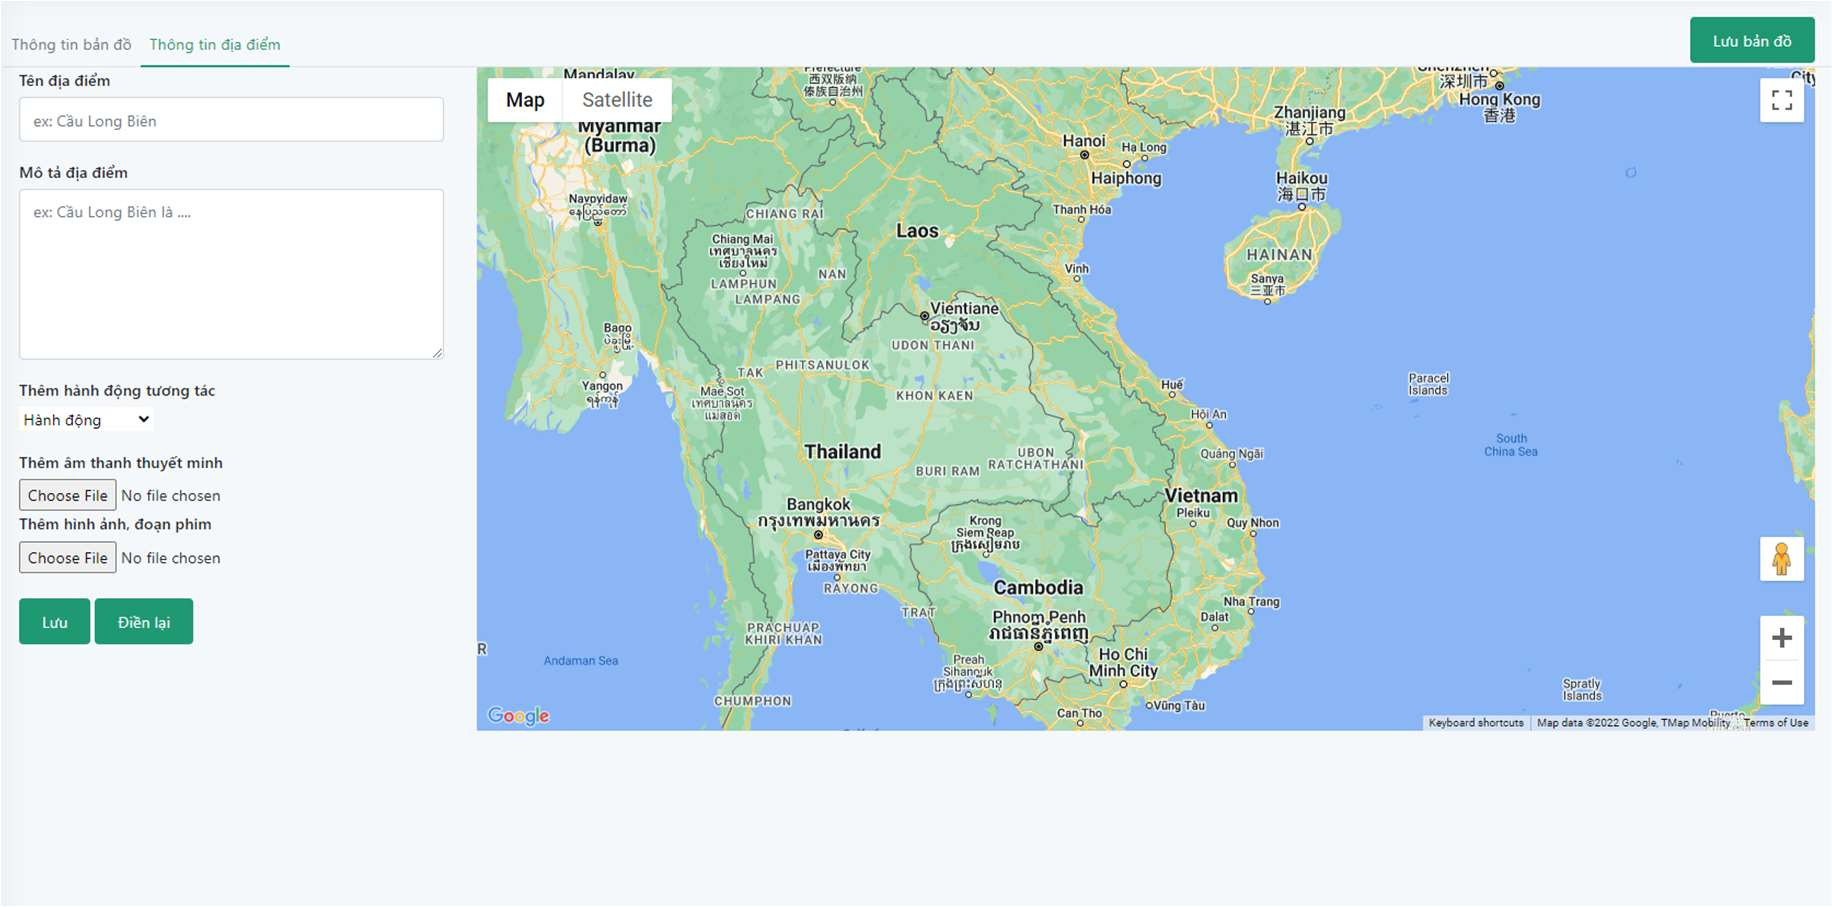
\includegraphics[width=0.8\textwidth]{figures/editor-point-info.jpg}
    \caption{Giao diện nhập thông tin chi tiết của điểm tham quan}
    \label{fig:editor-point-info}
\end{figure}

\begin{figure}[h]
    \centering
    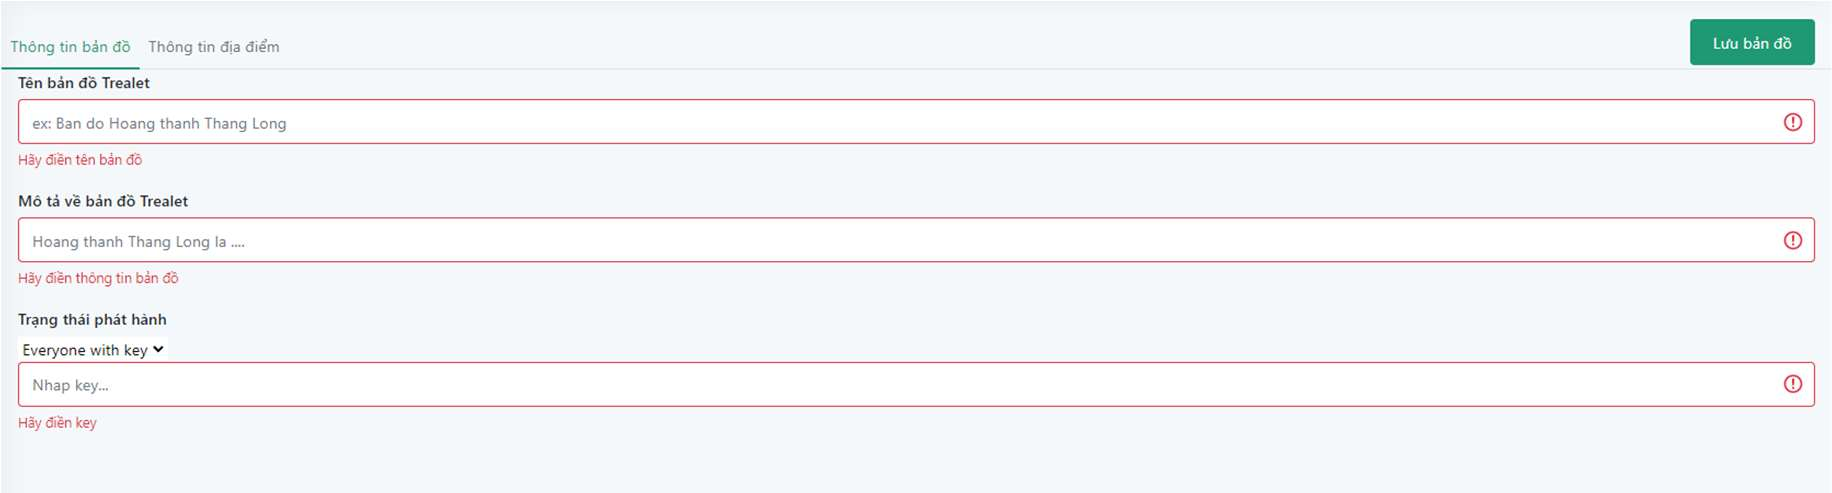
\includegraphics[width=0.8\textwidth]{figures/editor-map-password.jpg}
    \caption{Giao diện nhập mật khẩu cho Bản đồ}
    \label{fig:editor-map-password}
\end{figure}

\newpage
Ở màn hình thông tin chi tiết các địa điểm, người dùng chọn vị trí của địa điểm
trước khi điền các phần thông tin mô tả và tương tác. Khi người dùng cập nhật các
thông tin đa phương tiện, giao diện sẽ hiển thị lại thông tin đa phương tiện đó cho
người dùng để xem lại. Người dùng cũng sẽ thêm phần hành động tương tác với địa
điểm và mô tả cho hành động đó (\figurename~\ref{fig:editor-point-action}).

\begin{figure}[h]
    \centering
    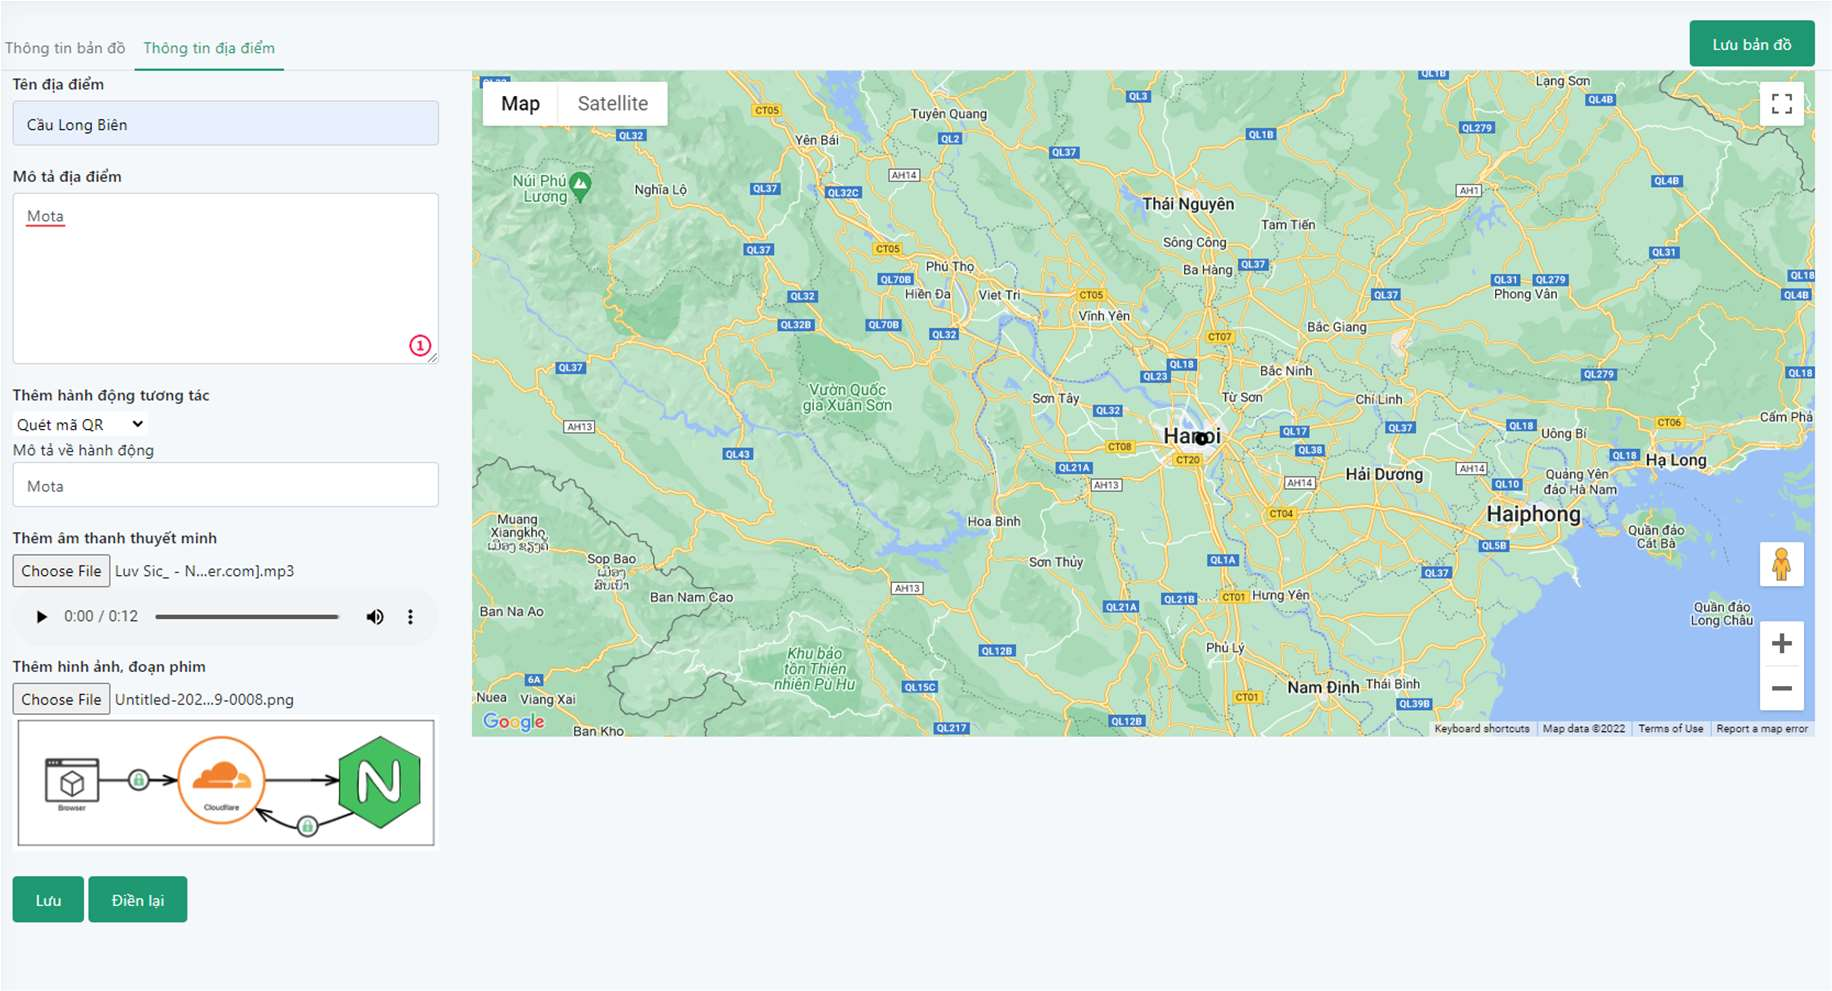
\includegraphics[width=0.8\textwidth]{figures/editor-point-action.jpg}
    \caption{Giao diện thêm hành động tương tác cho điểm tham quan}
    \label{fig:editor-point-action}
\end{figure}
Riêng phần hành động tương tác là “Thêm câu hỏi”, người dùng sẽ được cung
cấp một khung để nhập câu hỏi và bốn câu trả lời (\figurename~\ref{fig:editor-point-question}).

\begin{figure}[h]
    \centering
    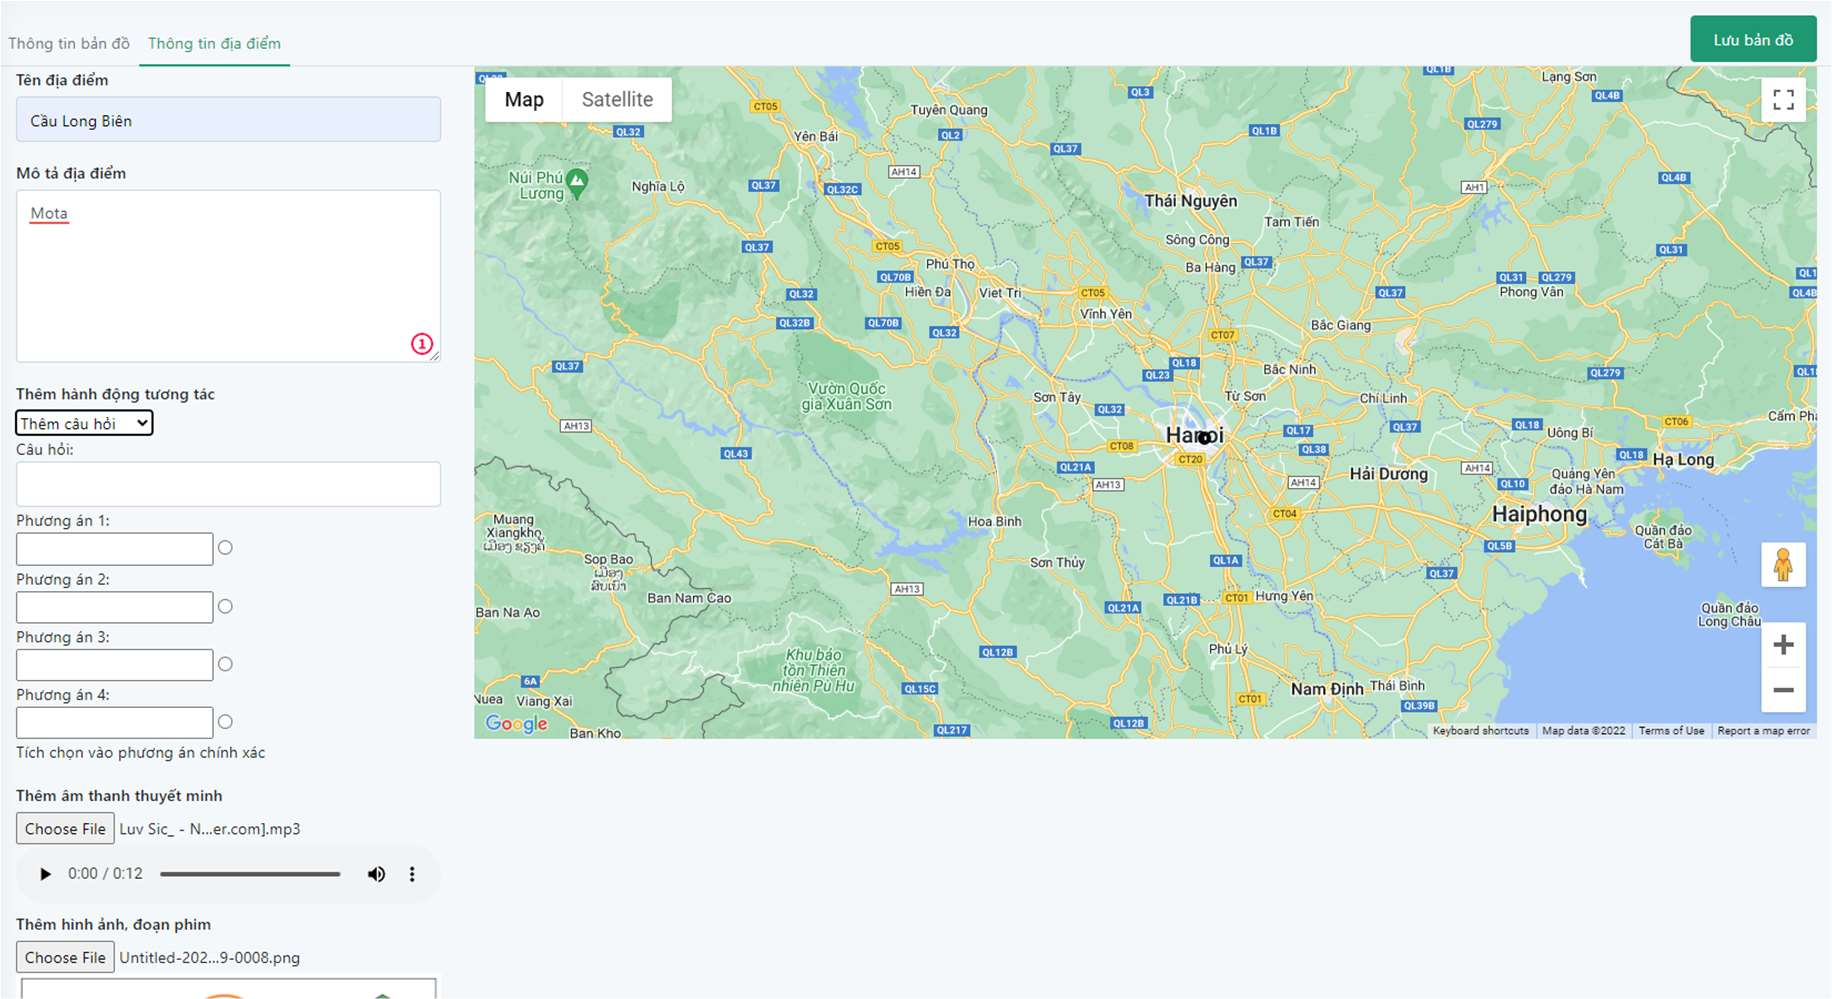
\includegraphics[width=0.8\textwidth]{figures/editor-point-question.jpg}
    \caption{Giao diện thêm câu hỏi cho điểm tham quan}
    \label{fig:editor-point-question}
\end{figure}
\newpage
Sau khi hoàn thiện các phần thông tin cần thiết, người dùng sẽ sử dụng nút lưu
để lưu lại thông tin tại điểm này, các điểm đã lưu sẽ được hiển thị trên bản đồ và có
thể sửa đổi được. Các điểm được thêm vào sẽ được đánh số lần lượt bắt đầu từ 1 (\figurename~\ref{fig:editor-point-number}).
\begin{figure}
    \centering
    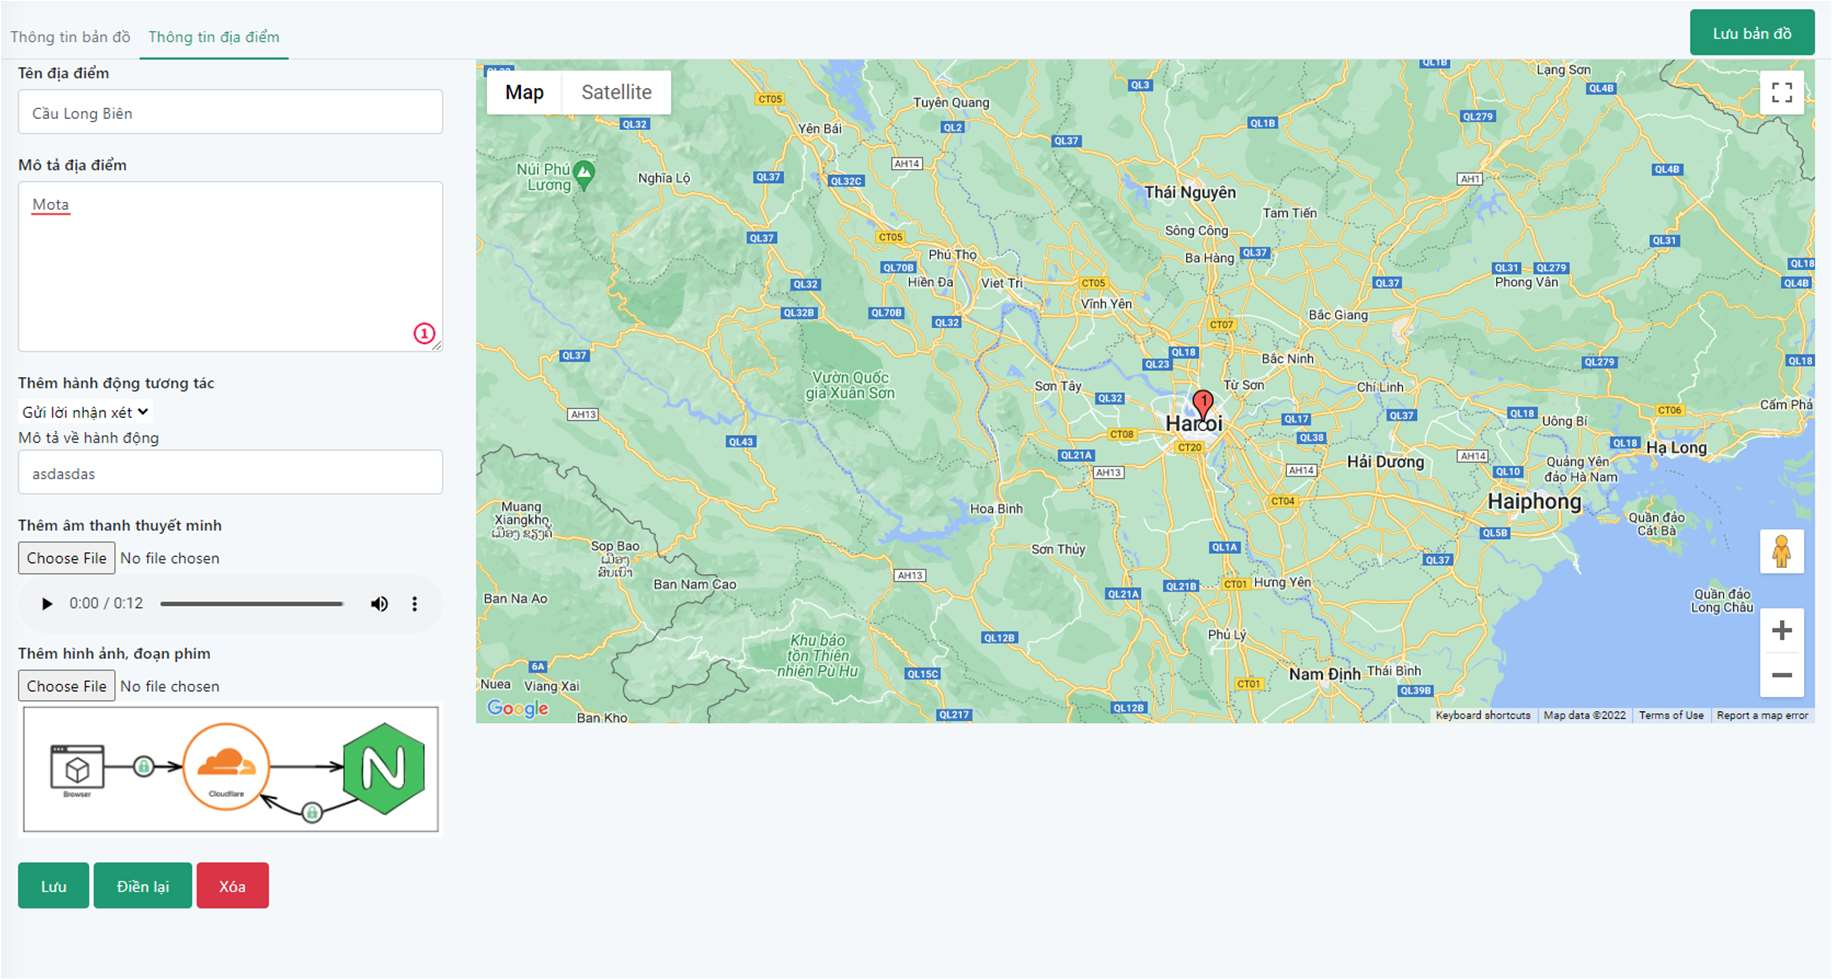
\includegraphics[width=0.8\textwidth]{figures/editor-point-number.jpg}
    \caption{Giao diện hiển thị các điểm tham quan đã thêm vào Bản đồ}
    \label{fig:editor-point-number}
\end{figure}
Sau khi hoàn thiện thông tin chung của bản đồ và thông tin chi tiết từng điểm,
người dùng ấn “Lưu bản đồ” và xác nhận để lưu bản đồ (\figurename~\ref{fig:editor-save-map}).
\begin{figure}[h]
    \centering
    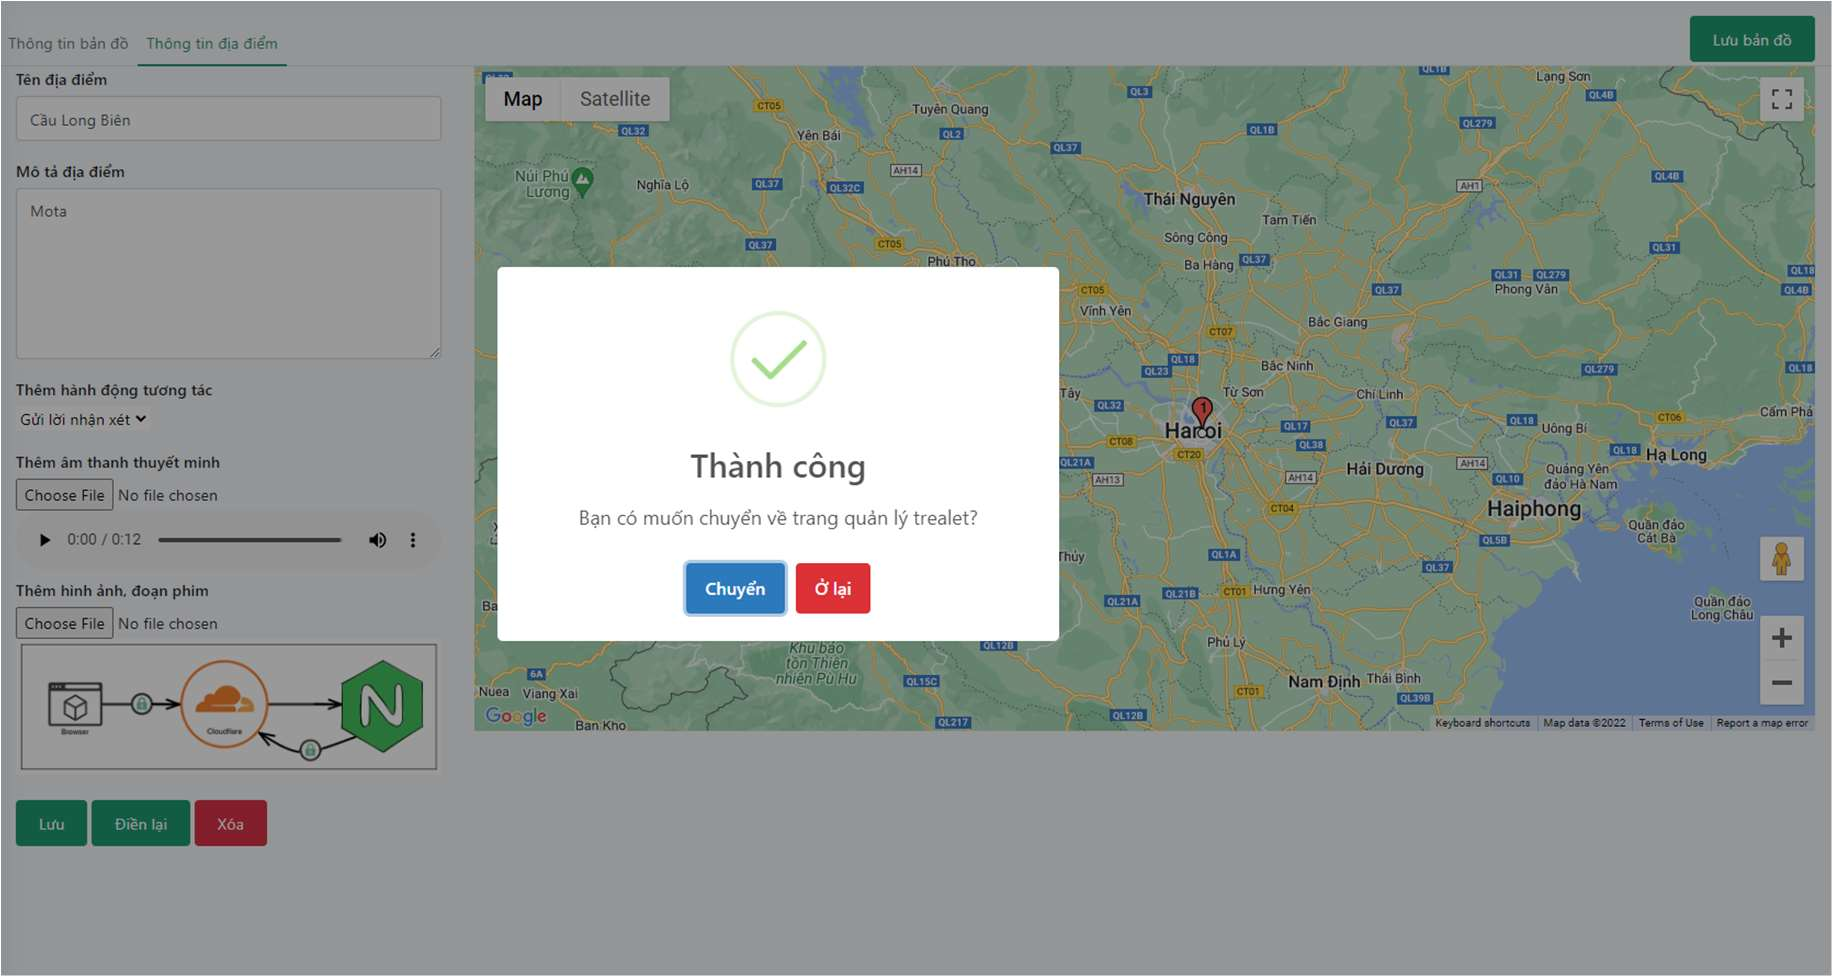
\includegraphics[width=0.8\textwidth]{figures/editor-save-map.jpg}
    \caption{Giao diện lưu Bản đồ}
    \label{fig:editor-save-map}
\end{figure}

\newpage
\textbf{Ứng dụng trải nghiệm}

Trang khởi đầu của Ứng dụng trải nghiệm sẽ là giao diện đăng nhập. Người
dùng có thể đăng nhập với email, mật khẩu, đăng nhập bằng tài khoản Google, đăng
ký tài khoản mới và thay đổi ngôn ngữ trong ứng dụng tại đây. \figurename~\ref{fig:player-login} mô tả màn hình trang chủ với khung đăng nhập thường và màn hình trang chủ với khung đăng
nhập bằng tài khoản Google.
\begin{figure}[h]
    \centering
    
\includegraphics[width=0.4\textwidth]{figures/player-login-1.jpg}
    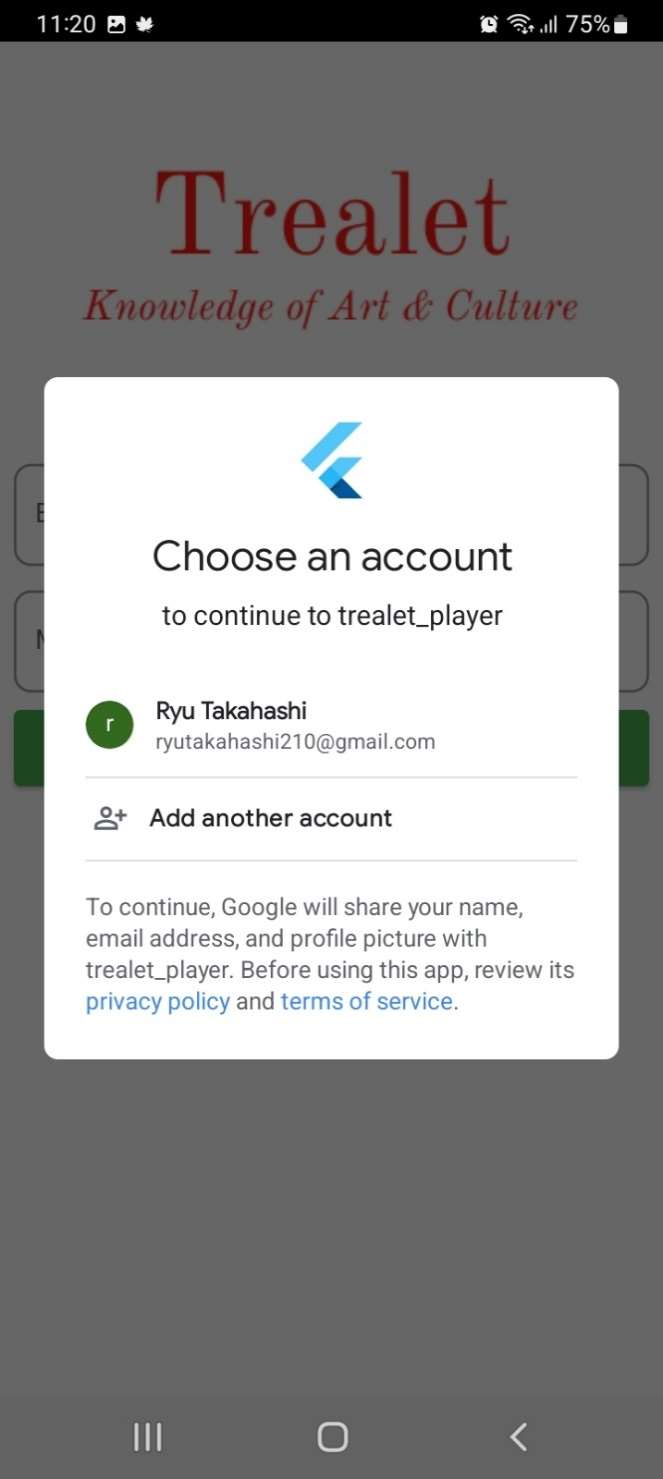
\includegraphics[width=0.4\textwidth]{figures/player-login-2.jpg}
    \caption{Giao diện đăng nhập của Ứng dụng trải nghiệm}
    \label{fig:player-login}
\end{figure}
Các tính năng trên trang chủ còn bao gồm nút đổi ngôn ngữ được đánh dấu
bởi quốc kỳ, nút đăng ký để chuyển người dùng đến giao diện đăng ký thông thường.
Trong giao diện đăng ký sẽ có bốn khung để người dùng nhập tên người dùng, email,
nhập mật khẩu và nhập lại mật khẩu (\figurename~\ref{fig:player-register}). Trong trường hợp người dùng nhập thông tin vào đơn đăng ký sai định dạng
quy định, như tên người dùng trùng, email sai định dạng, để trống mật khẩu, hệ thống
sẽ báo lỗi lại để người dùng sửa.
\begin{figure}
    \centering
    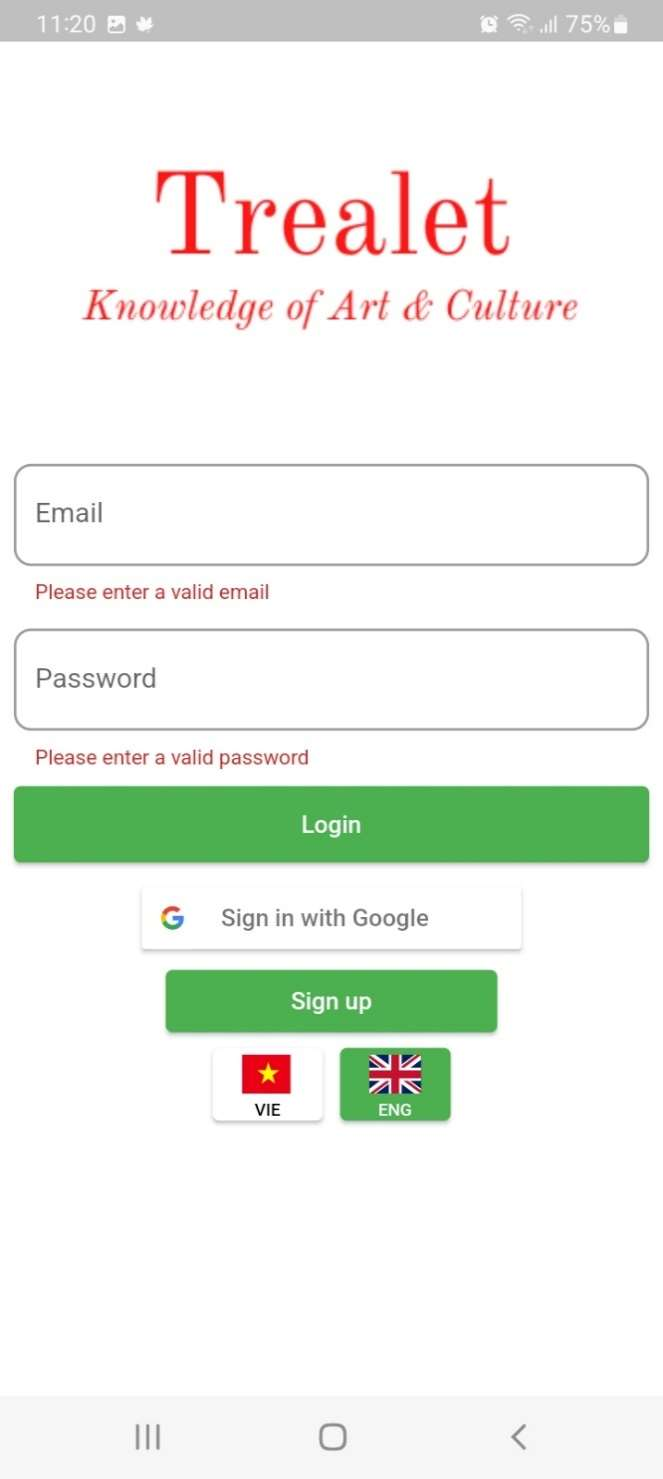
\includegraphics[width=0.4\textwidth]{figures/player-register-1.jpg}
    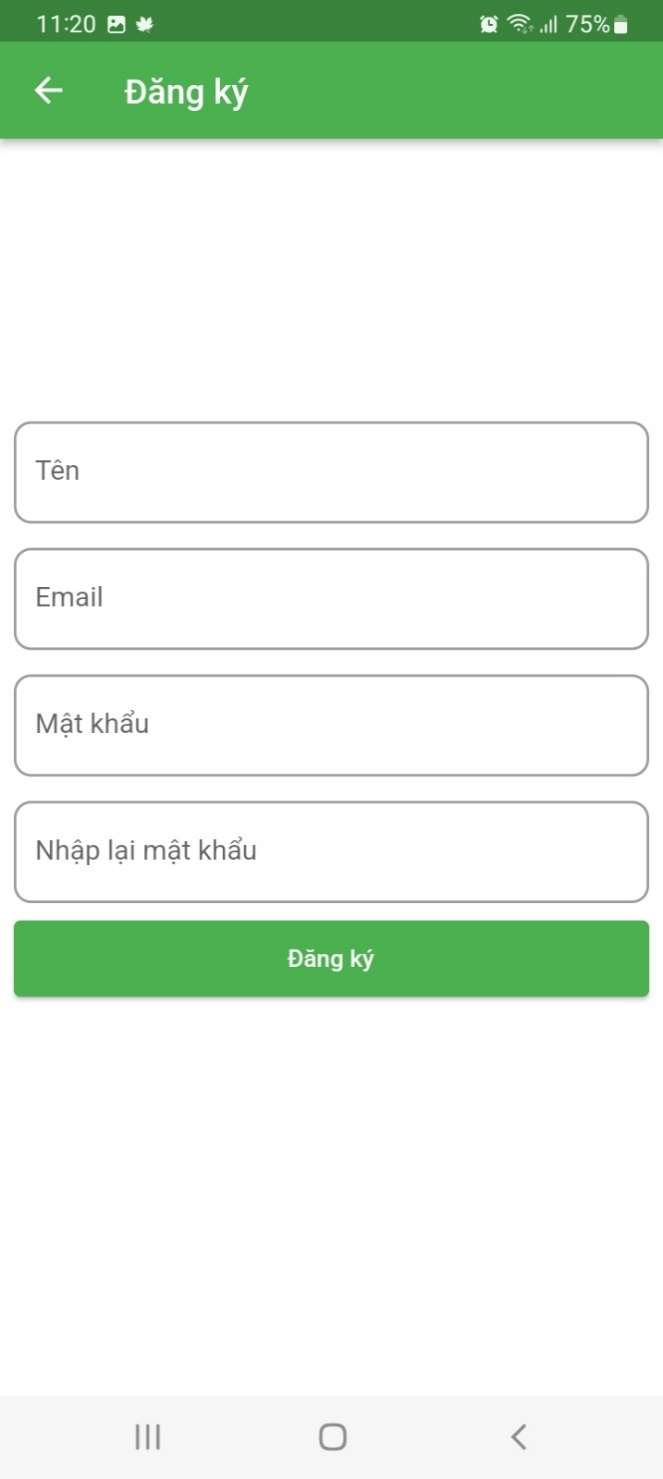
\includegraphics[width=0.4\textwidth]{figures/player-register-2.jpg}
    \caption{Giao diện đăng ký của Ứng dụng trải nghiệm}
    \label{fig:player-register}
\end{figure}

\newpage
Sau khi đăng nhập thành công, Ứng dụng trải nghiệm hiển thị màn hình danh
sách các bản đồ để trải nghiệm cùng với thanh tìm kiếm, màn hình có bao gồm một
thanh kéo bên trái để đăng xuất và tải lại danh sách Bản đồ như trong \figurename~\ref{fig:player-map-list}.
\begin{figure}
    \centering
    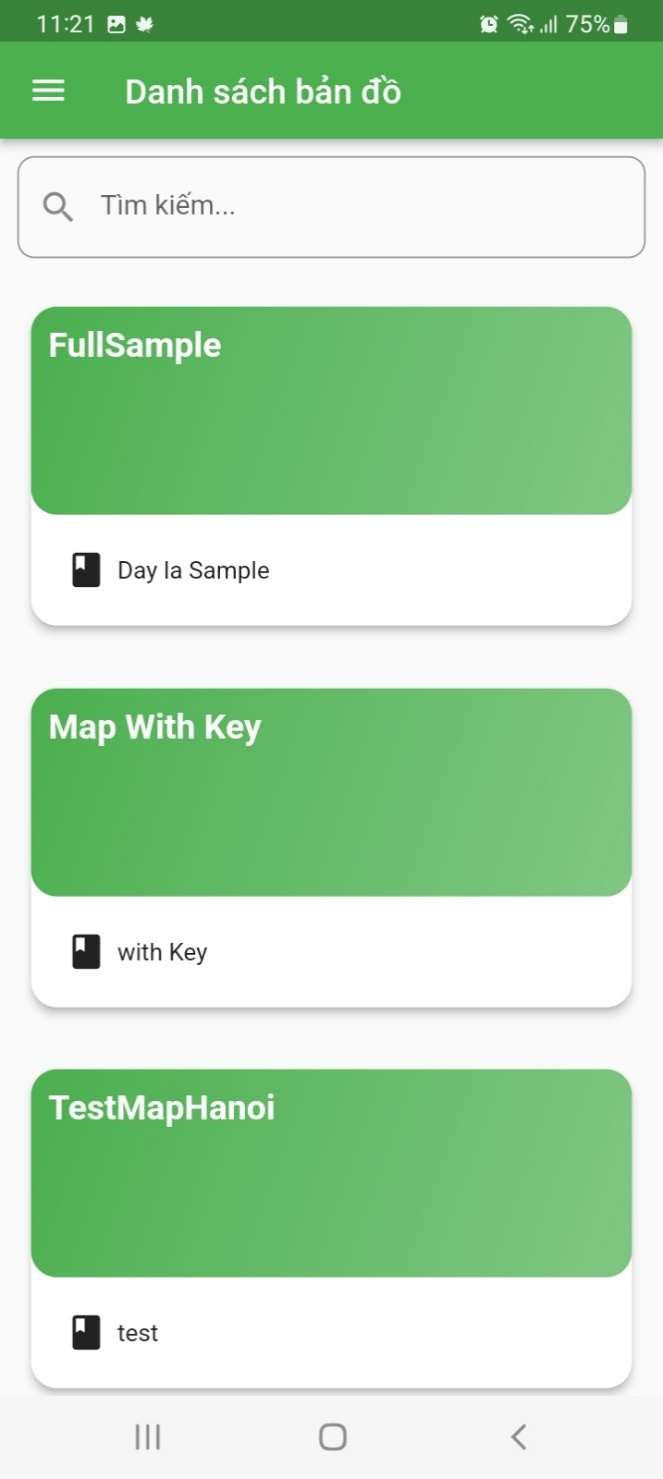
\includegraphics[width=0.4\textwidth]{figures/player-map-list-1.jpg}
    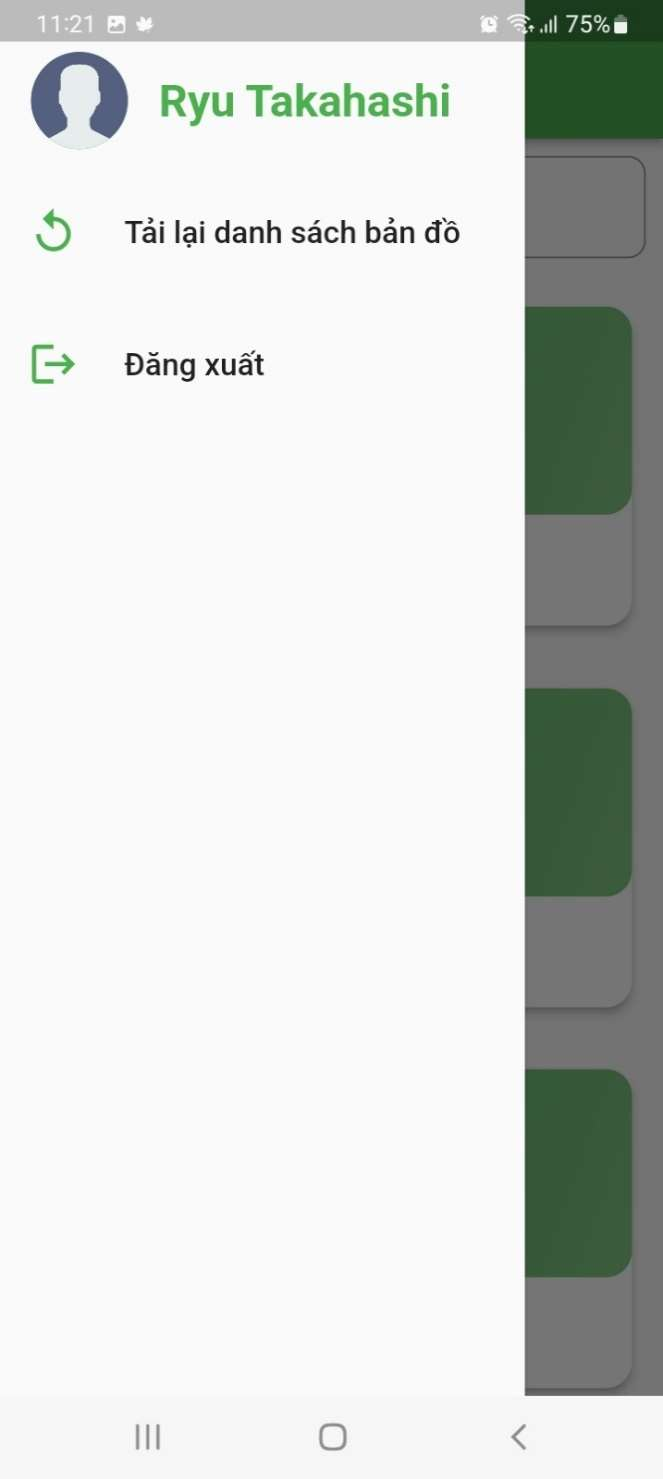
\includegraphics[width=0.4\textwidth]{figures/player-map-list-2.jpg}
    \caption{Giao diện danh sách Bản đồ của Ứng dụng trải nghiệm}
    \label{fig:player-map-list}
\end{figure}

Khi người dùng chọn Bản đồ, trong trường hợp Bản đồ có yêu cầu mật khẩu, người
dùng sẽ được cung cấp một khung để nhập mật khẩu Bản đồ. Sau khi xác nhận vào Bản đồ
thành công bằng mật khẩu hoặc vào một Bản đồ không có mật khẩu, Ứng dụng trải
nghiệm hiển thị bản đồ và vị trí hiện tại của người dùng. Bên trên là một thanh thông
báo khoảng cách của người dùng đến điểm trải nghiệm tiếp theo. Trong màn hình bản
đồ hiển thị các điểm tham quan với các ô tròn màu xám được đánh số theo số thứ tự
đã được người sáng tạo khai báo khi tạo bản đồ. Người dùng cũng có thể tìm vị trí của bản thân hay phóng lớn thu nhỏ bản đồ bằng các nút nằm ở góc phải trên và góc
phải dưới của màn hình \figurename~\ref{fig:player-in-map}.
\begin{figure}[h]
    \centering
    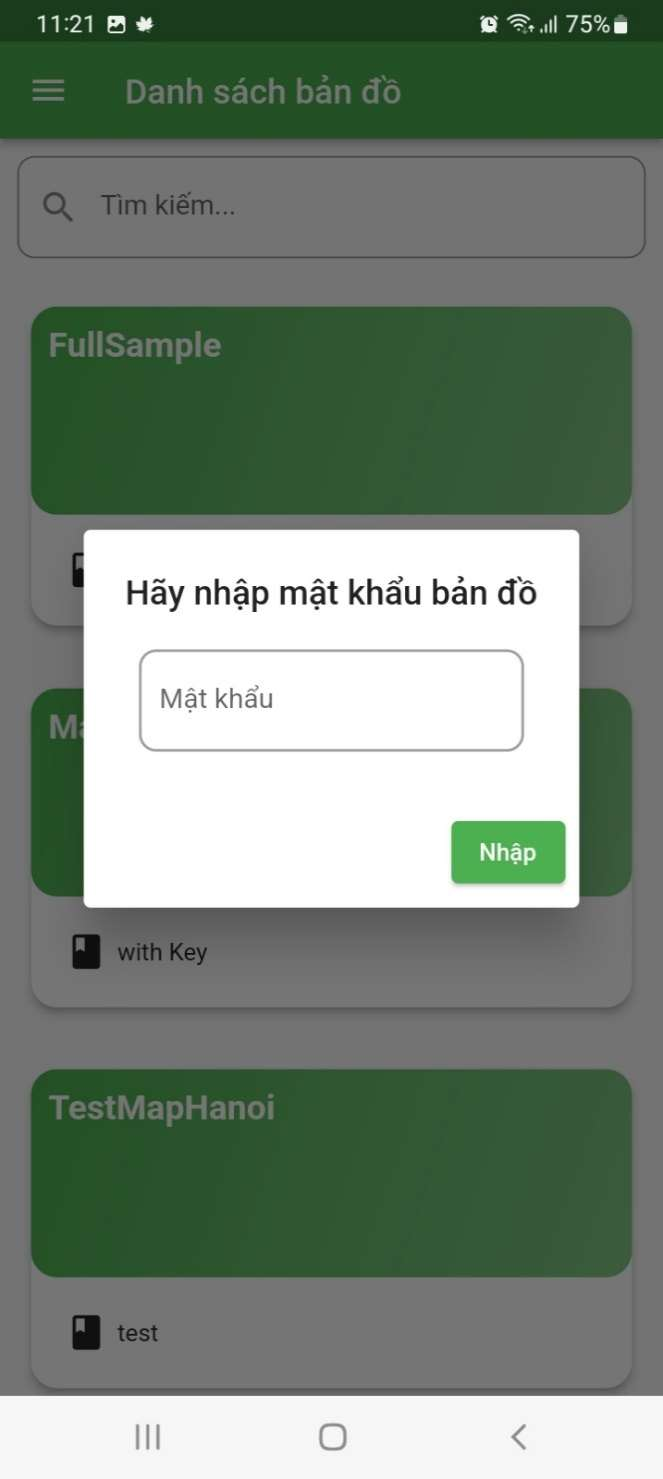
\includegraphics[width=0.4\textwidth]{figures/player-in-map-1.jpg}
    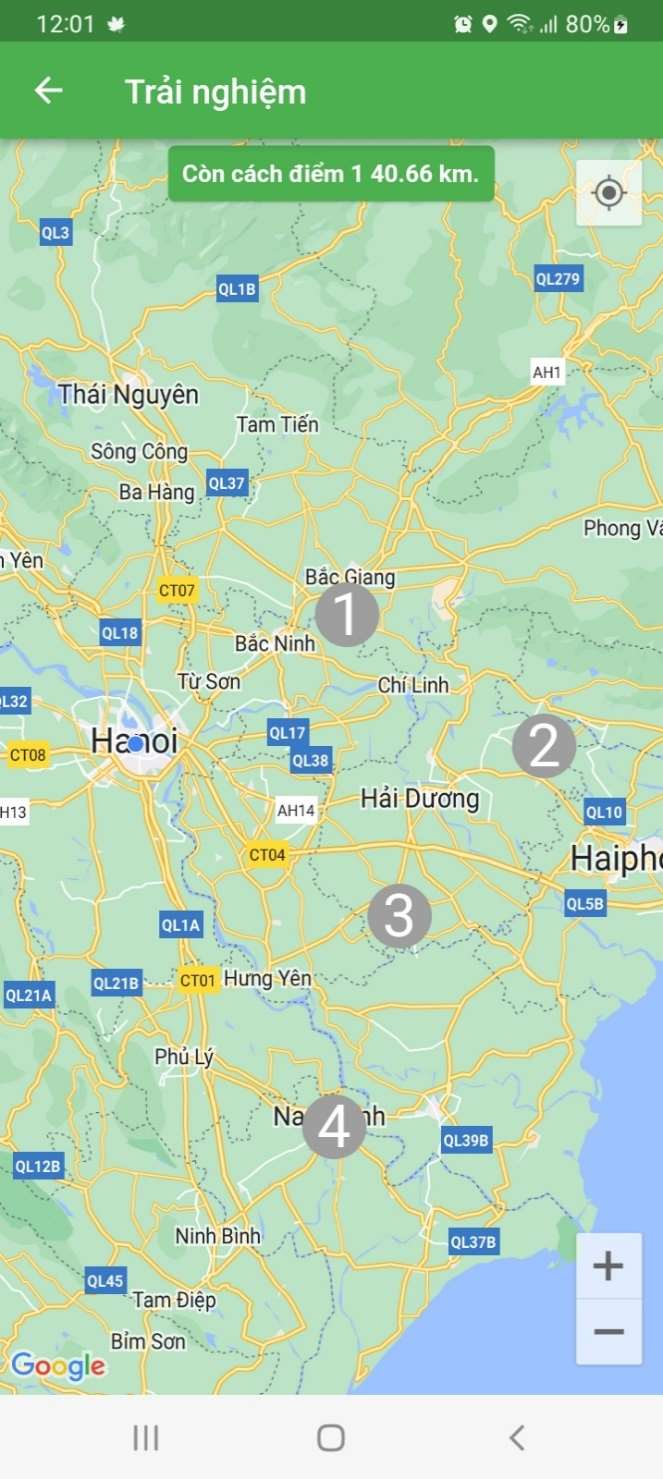
\includegraphics[width=0.4\textwidth]{figures/player-in-map-2.jpg}
    \caption{Giao diện trải nghiệm Bản đồ của Ứng dụng trải nghiệm}
    \label{fig:player-in-map}
\end{figure}

Trên bản đồ, các điểm chưa được lưu trữ tương tác sẽ có màu xám, trong khi
các điểm đã tương tác sẽ có màu xanh. Các điểm này sẽ hiện một tiêu đề khi chạm
vào. Người dùng chọn tiêu đề này để xem nội dung mô tả của điểm tham quan, cũng
như tương tác với chúng (\figurename~\ref{fig:player-interaction}).

\begin{figure}
    \centering
    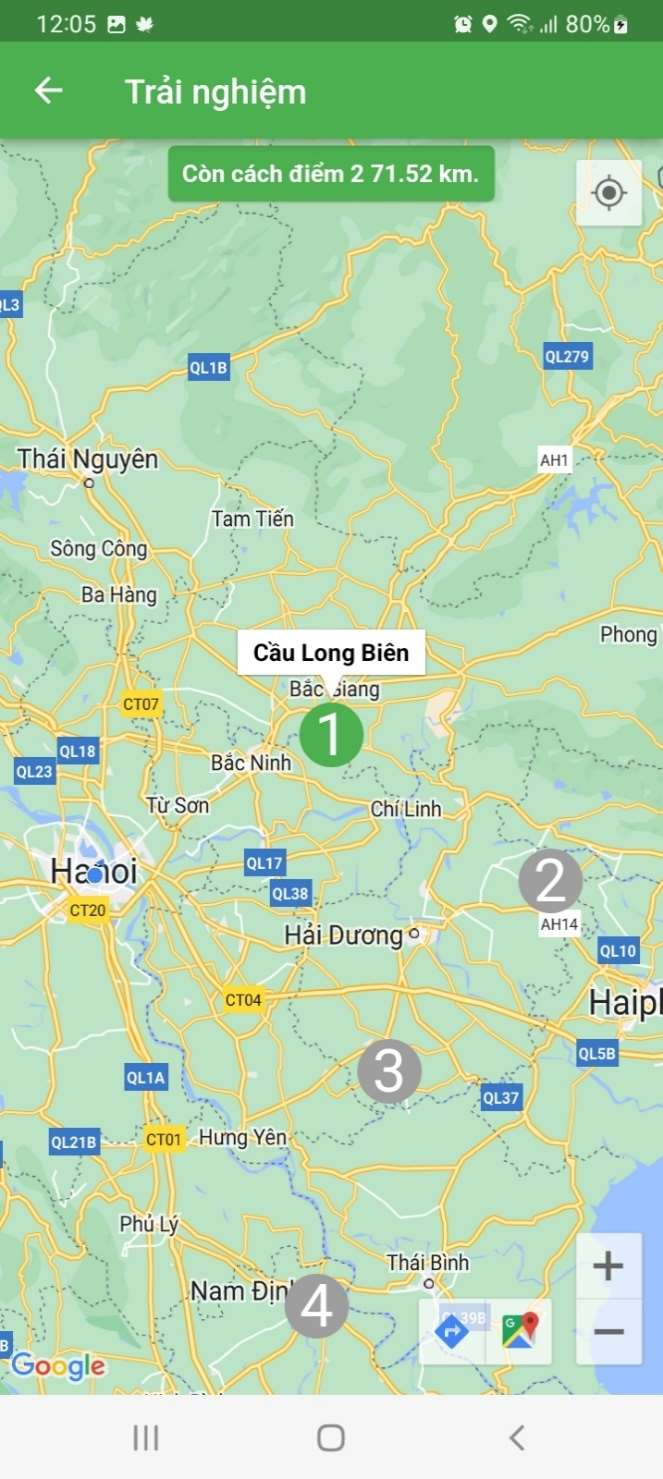
\includegraphics[width=0.4\textwidth]{figures/player-interaction-1.jpg}
    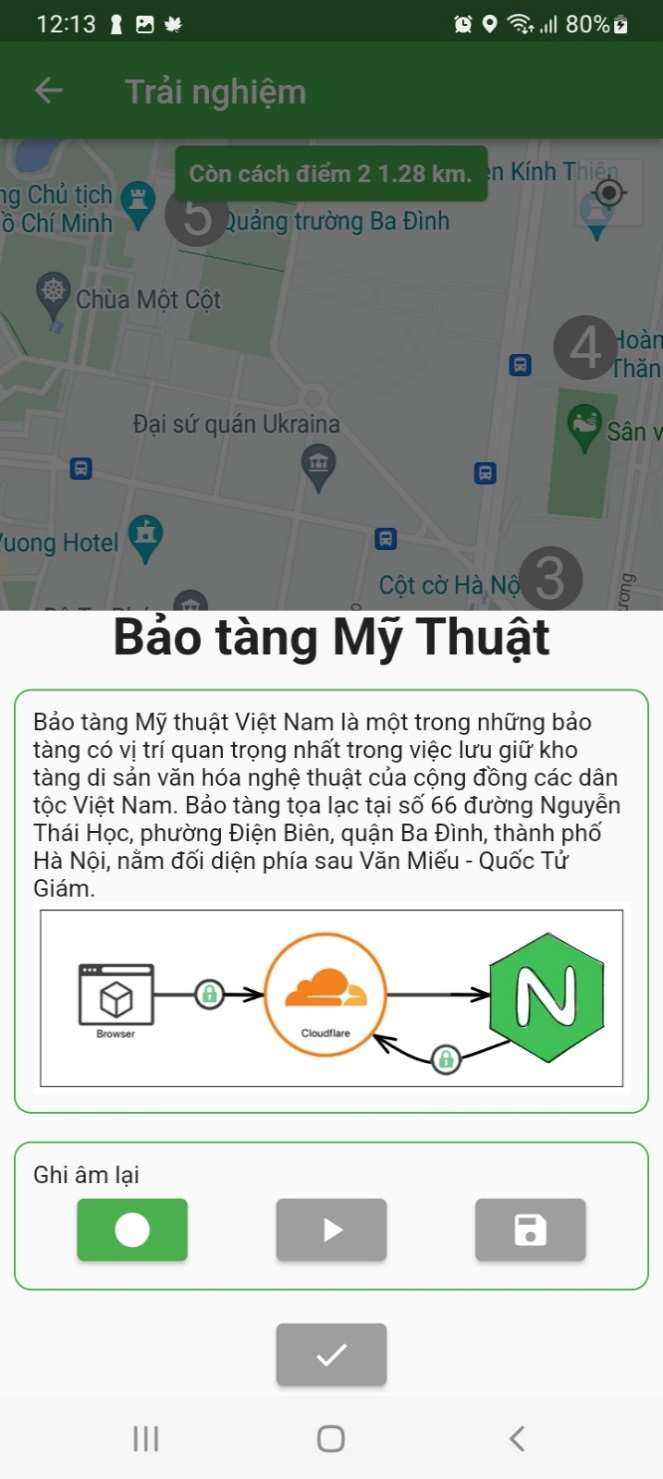
\includegraphics[width=0.4\textwidth]{figures/player-interaction-2.jpg}
    \caption{Giao diện tương tác điểm tham quan của Ứng dụng trải nghiệm}
    \label{fig:player-interaction}
\end{figure}

\newpage
\section{Cài đặt và tích hợp ứng dụng}
\subsection{Phần Server và Trình biên soạn}
\textbf{Thiết lập môi trường phát triển}

Môi trường phát triển của phần server và trình biên soạn cần có framework PHP
Laravel, trình quản lý gói Composer. Do tập mã nguồn này được tích hợp chung với
hệ thống chung Trealet, cần tải xuống tập mã nguồn đã được tích hợp sẵn các
thông tin kết nối với cơ sở dữ liệu chung, từ đó có thể bắt đầu phát triển, đồng thời tái sử dụng lại các phần module có thể dùng chung trong hệ thống sẵn có, như module
đăng tải file dữ liệu, module xử lý truy vấn cơ sở dữ liệu, …

\textbf{Lập trình}

Bắt đầu với việc khai báo các controller cần thiết trong phần định hướng của
tập mã nguồn. Với các đường dẫn tương ứng, khai báo hàm xử lý cho yêu cầu tới
đường dẫn đó, và thực hiện lập trình hàm này trong một tập tin controller riêng. Phần
controller của Trình biên soạn, bao gồm hiển thị trang biên soạn bản đồ, API nhận
yêu cầu lưu bản đồ, trong đó phần trang biên soạn bản đồ, cần bổ sung thêm phần
giao diện được viết bởi Blade template, kết hợp cú pháp của PHP, HTML và
JavaScript.
Tương tự với Server, cần khai báo và thực thi Controller chứa các API phục
vụ cho ứng dụng trải nghiệm, bao gồm API lấy tất cả các bản đồ, đăng nhập, đăng
ký, lấy chi tiết bản đồ, lưu lại tương tác của người chơi.

\textbf{Triển khai}

Phần triển khai đã được tận dụng lại luồng triển khai thông qua Gitlab CI và
Docker Compose của hệ thống Trealet. Hệ thống sau khi triển khai có thể được truy
cập với tên miền trealet.com.

\subsection{Phần Ứng dụng trải nghiệm}

\textbf{Thiết lập môi trường phát triển}

Ứng dụng trải nghiệm được phát triển bằng ngôn ngữ Dart trên framework là
Flutter, thiết lập Flutter và Android Studio để tạo ra môi trường phát triển
bao gồm phần framework với các module để lập trình, Android Studio có chứa các
máy ảo phục vụ cho việc chạy thử và gỡ lỗi chương trình trong phát triển.

\textbf{Lập trình}

Lập trình ứng dụng này, bắt đầu với việc khai báo các module phụ thuộc để
phục vụ cho mục đích quản lý trạng thái dữ liệu về bản đồ, người dùng, ngôn ngữ
hiện tại của ứng dụng, các module về tính năng như trình chạy nội dung đa phương
tiện, bộ xin quyền hệ thống để truy cập vào máy ảnh, microphone của điện thoại và
module bản đồ để xây dựng phần trải nghiệm.
Sau khi đã khai báo và cài đặt thành công các module này, tiến hành viết mã
nguồn với cấu trúc tập mã nguồn được chia làm 3 phần chính: Phần dữ liệu chung
của ứng dụng, các trang màn hình và các thành phần giao diện được tách riêng để tái sử dụng. Ngoài cùng sẽ có một tập mã nguồn chính làm điểm khởi đầu cho ứng dụng.
Tập mã nguồn chính sẽ chứa thông tin điều hướng đến các trang màn hình, khởi tạo
luồng dữ liệu cho các trang này. Các trang màn hình có thể tận dụng dữ liệu, dựng
lên các thành phần giao diện riêng hoặc tái sử dụng các thành phần giao diện đã được
tách ra.

\textbf{Đóng gói}
Đóng gói ứng dụng ra tập tin apk bằng hỗ trợ của framework Flutter, với câu
lệnh flutter build apk.

\section{Thử nghiệm ứng dụng TMAP}
\subsection{Thử nghiệm}
Với năm địa điểm là Văn
Miếu – Quốc Tử Giám, Nhà tù Hỏa Lò, Hoàng thành Thăng Long, Lăng Chủ tịch Hồ
Chí Minh và Bảo Tàng Hồ Chí Minh, xây dựng kịch bản thử nghiệm với nội dung
cụ thể như sau:

\textbf{Tên bản đồ:} Hà Nội

\textbf{Mô tả:} Khám phá Hà Nội

\textbf{Hình thức phát hành:} Phát hành cho tất cả với mật khẩu là “hanoi”

Nội dung các điểm tham quan được mô tả trong \tablename~\ref{tab:test-map-content}.
\begin{table}[h]
\centering
\caption{Nội dung các điểm tham quan trong bản đồ thử nghiệm}
\label{tab:test-map-content}
\begin{tabular}{|p{3cm}|p{6cm}|p{5cm}|}
\hline
\textbf{Tên địa điểm} & \textbf{Mô tả} & \textbf{Tương tác} \\ \hline
Văn Miếu - Quốc
Tử Giám
&Văn bản đính
kèm ảnh
&Hình thức: Chụp ảnh \newline
Mô tả: Hãy chụp lại Khuê Văn Các \\ \hline
Nhà tù Hỏa Lò
&Văn bản đính
kèm video
&Hình thức: Ghi âm \newline
Mô tả: Ghi âm thuyết minh \\ \hline
Hoàng thành
Thăng Long
&Văn bản đính
kèm ảnh
&Hình thức: Quét mã QR \newline
Mô tả: Quét mã QR thông tin \\ \hline
Lăng Chủ tịch
Hồ Chí Minh
&Văn bản đính
kèm ảnh
&Hình thức: Gửi lời nhận xét \newline
Mô tả: Nhận xét về địa điểm \\ \hline
Bảo Tàng
Hồ Chí Minh
& Văn bản đính
kèm ảnh
&Hình thức: Trả lời câu hỏi \newline
Mô tả: Bảo tang Hồ Chí Minh được thành lập vào năm bao nhiêu? \\ \hline
\end{tabular}
\end{table}
\newpage
Kết quả kịch bản hiển thị trên ứng dụng trải nghiệm thể hiện đầy đủ năm điểm tham
quan với tọa độ thực trên Google Map. Mỗi điểm có thông tin mô tả như đã nhập
trên trình biên soạn \figurename~\ref{fig:test-map-points}. 

\begin{figure}[h]
    \centering
    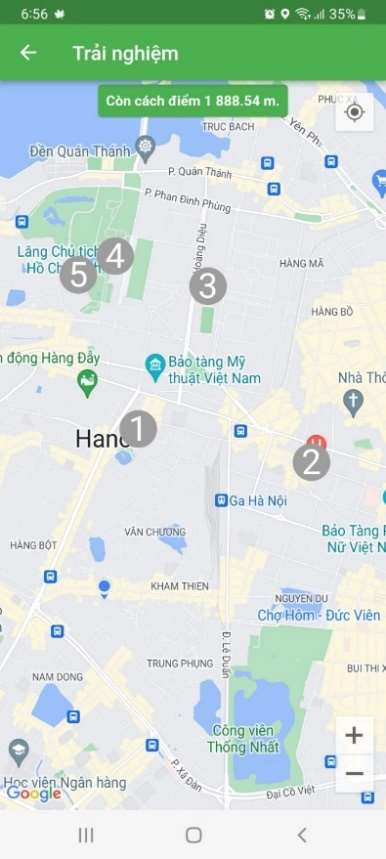
\includegraphics[width=0.4\textwidth]{figures/test-map-points-1.jpg}
    
\includegraphics[width=0.4\textwidth]{figures/test-map-points-2.jpg}
    \caption{Giao diện trải nghiệm bản đồ thử nghiệm với năm điểm tham quan}
    \label{fig:test-map-points}
\end{figure}
\newpage
\subsection{Kết quả thử nghiệm}
Về tính năng, TMAP hiện tại đã đáp ứng được các yêu cầu của bài toán đã đề
ra. Trình biên soạn đã hỗ trợ các tính năng thiết yếu như chọn điền mô tả bản đồ, chọn
địa điểm, điền mô tả địa điểm và đăng tải nội dung đa phương tiện cùng với bổ sung
tương tác, tuy nhiên lượng hình thức tương tác còn ít. Ứng dụng trải nghiệm thể hiện
lại chính xác nội dung bản đồ đã được tạo ra, ghi và lưu lại thành công các tương tác
của người trải nghiệm trên bản đồ. Thông tin vị trí và khoảng cách tới các điểm cũng
được đo lường liên tục với sai số chấp nhận được.

Về giao diện, trình biên soạn đã cung cấp giao diện đơn giản và dễ sử dụng
với khung bản đồ và các khung điền thông tin. Tuy nhiên về ứng dụng trải nghiệm,
việc thể hiện danh sách các bản đồ còn đơn giản ở dạng cột dọc, chưa có sự hấp dẫn
cũng như thể hiện được tính đa dạng của các loại bản đồ. Các màu được sử dụng còn
đơn giản, chưa bắt mắt hay gây được nhiều hứng thú cho người trải nghiệm.

Về khả năng mở rộng, với những thiếu sót đã trình bày ở trên, cả hai phần trình
biên soạn và ứng dụng trải nghiệm đều có thể được phát triển tốt hơn nữa. Trình biên
soạn cần được bổ sung thêm về các hình thức tương tác đa dạng hơn, và giao diện
của ứng dụng trải nghiệm cần được trau chuốt tỉ mỉ và gây hứng thú hơn cho người
sử dụng.\newpage\cleardoublepage         % Chương 3: Phương pháp & Thiết kế
% \begin{center}
\textbf{\large{Kết luận}	}
\end{center}
\addcontentsline{toc}{chapter}{Kết luận}

\textbf{Kết quả đạt được}

Khóa luận đã hoàn thành phát triển hệ thống TMAP với
hai phần là trình biên soạn trên Website và ứng dụng trải nghiệm trên điện thoại. Phần
trình biên soạn đã được triển khai và có thể được sử dụng trên các trình duyệt phổ
thông, đáp ứng được nhu cầu tạo trải nghiệm của các đơn vị văn hóa. Phần ứng dụng
trải nghiệm đã được đóng gói và có thể sẵn sàng phát hành cho đông đảo người sử
dụng. TMAP qua đó đã đáp ứng được những đầu mục cơ bản của bản đồ số trong du
lịch văn hóa, hỗ trợ được phần nào trải nghiệm của du khách trong quá trình khám
phá các địa điểm du lịch.

Ứng dụng cũng đóng góp một phần nhỏ trong quá trình hoàn thiện dự án lớn
Trealet, tham gia vào xu hướng ứng dụng công nghệ thông tin để quảng bá và giáo
dục văn hóa du lịch đang ngày càng lớn mạnh. Kết quả của khóa luận sẽ được ứng
dụng tại Bảo tàng Văn hóa các Dân tộc Việt Nam ở Thái Nguyên.

\textbf{Hướng phát triển}

Các hình thức tương tác và mô tả điểm du lịch của TMAP
có nhiều tiềm năng để phát triển đa dạng hơn, bên cạnh đó phần giao diện vẫn còn
đơn giản sẽ là những ưu tiên đầu trong việc sửa đổi và phát triển TMAP. Hi vọng có thể biến TMAP thành sản
phẩm có thể được sử dụng rộng rãi trong truyền bá, giáo dục các địa điểm văn hóa.\newpage\cleardoublepage    % Chương 4: Thực nghiệm & Công cụ
% \input{chapters/c5_conclusion}\newpage\cleardoublepage     % Chương 5: Kết luận & Hướng phát triển

% \phantomsection 
% \addcontentsline{toc}{chapter}{Tài liệu tham khảo}
% \bibliography{references}\newpage\cleardoublepage
% \bibliographystyle{plain}

% \appendix
% \input{chapters/appendix}\newpage\cleardoublepage

\end{document}
